\documentclass[11pt]{book}

\usepackage{geometry}
\usepackage{framed}
\usepackage{graphicx}

\usepackage[T1]{fontenc}
\usepackage{tgtermes}    % body font
\usepackage{inconsolata} % fixed width font
\usepackage{tgheros}     % sans-serif font

\author{Greg Wilson}

\geometry{
  paperwidth=18.91cm,
  paperheight=24.589cm,
  vmargin=1.9cm, % top and bottom margins
  inner=1.9cm, % inside margin
  outer=2.29cm, % outside margin
  bindingoffset=0.89cm % gutter
}

\setcounter{tocdepth}{0}    % sets what level of header is shown in the TOC
\setcounter{secnumdepth}{1} % sets what level of subsect. are numbered

\newenvironment{boxedsection}[3]
{\begin{figure}[h!]\vspace{-0.7cm}\centering \rule[-.7cm]{12.82cm}{0.75pt} \begin{minipage}[t]{12.82cm}\begin{framed}\centerline{{\textbf{{#1}: #2}}}}
{\end{framed}\end{minipage} \rule{12.82cm}{0.75pt} \end{figure}}

\newenvironment{callout}[2]{\begin{boxedsection}{Callout}{#1}{#2} }{ \end{boxedsection}}
\newenvironment{checklist}[2]{\begin{boxedsection}{Checklist}{#1}{#2} }{ \end{boxedsection}}
\newenvironment{challenge}[2]{\begin{boxedsection}{Challenge}{#1}{#2} }{ \end{boxedsection}}
\newenvironment{discussion}[2]{\begin{boxedsection}{Discussion}{#1}{#2} }{ \end{boxedsection}}

\newcommand{\figlbl}[4][375pt]{\begin{figure}\centering\includegraphics[width={#1}]{#2}\label{#3}\caption{#4}\end{figure}}

\newcommand{\chaplbl}[2]{\chapter{#1}\label{#2}}
\newcommand{\chapref}[1]{Chapter~\ref{#1}}
\newcommand{\href}[2]{#2\footnote{#1}}
\newcommand{\seclbl}[2]{\section{#1}\label{#2}}
\newcommand{\secref}[1]{Section~\ref{#1}}

\title{A Short Guide to Teaching}
\date{}

\raggedbottom

\begin{document}
\tableofcontents

\chaplbltime{Introductions}{sec:welcome}{15}{15}

There's more to programming than typing in code.  Good programmers
break their software up into functions, automate repetitive tasks, and
keep track of their work using version control.  Once they have
mastered those basics, they start doing code reviews and writing tests
as they go along.  They don't invent these techniques for themselves:
more experienced programmers teach them (either explicitly or by
example), and they in turn pass them on to others.

Similarly, there's more to teaching than talking.  Good teachers break
subjects up into digestible pieces, design lessons with verifiable
goals in mind, check their students' progress at short intervals, and
encourage collaboration and improvisation.  Like good programming
practices, these don't have to be reinvented by every teacher: they
can and should be taught and learned.  And while they can't
automatically make someone a great teacher, they do make people better
teachers.

This training course is a fast, wide-ranging, and (necessarily)
incomplete introduction to modern evidence-based teaching practices.
Its aim is introduce you to what we actually know about teaching and
learning, why we believe it is true, and how you can apply it.  We
will look at:

\begin{itemize}

\item
  how people's thinking changes as they go from being novices to
  competent practitioners and then to being experts;

\item
  how to tell if your learners are keeping up with you, and what to
  do or say when they're not;

\item
  how to design and improve lessons efficiently and collaboratively;

\item
  how and why live coding is a better way to teach programming than
  lectures or self-directed practice; and

\item
  how insights and techniques borrowed from the performing arts can
  make you a better teacher.

\end{itemize}

We can't cover everything you need to know to teach well.  In fact,
we can barely scratch the surface.  But we hope that what we show you
will be useful, and will convince you that better is possible.

\section*{History}

I started teaching people how to program in the late 1980s.  At first,
I was pretty bad at: I went too fast, I used too much jargon, and I
assumed that my learners would be interested in the same things I was.
I got better over time, but that doesn't mean I was actually very
good.  And even though I felt I was improving, I had no idea how
effective I was compared to other teachers.

My doubts came to a head after I re-launched Software Carpentry in
2010.  Its aim was (and is) to teach basic computing skills to
researchers from a wide range of disciplines.  What I realized then
was that, ironically, I was trying to teach people how to build and
run software in efficient, repeatable ways, but was mostly ignorant of
equivalent techniques for writing and delivering lessons.

Luckily, I discovered resources like Mark Guzdial's blog
\cite{bib:guzdial-blog} and the book \emph{How Learning
Works} \cite{bib:ambrose-hlw}.  These led me to the work of Lemov,
Huston, Green, and others
\cite{bib:lemov-champion,bib:huston-dont-know,bib:green-babt},
which showed me what would make my teaching better, and why I should
believe it.

I started using these ideas in Software Carpentry in 2012, and the
results were everything I'd hoped for.  Cutting the number of lessons,
shifting to in-person delivery, and using live coding all had an
impact.  What made the biggest difference, though, was creating a
training course to turn learners into teachers.

While I originally delivered the course online over multiple weeks, by
2014 I was teaching it in two intensive days, just like our regular
software skills workshops.  A year later, ``I'' became ``we'' as
people who had taught regular workshops began training new instructors
as well.  That same year, I began teaching half-day and one-day
versions of the course to people who wanted to help children, recent
immigrants, women re-entering the workforce, and a wide variety of
others.

Those experiences are the basis of this book, but its roots go much
deeper.  I am grateful, always, to Louis Biczo, Lon Taylor, Ken
Douglas, and above all, my father, Rob Wilson, for starting me down
this path.  I am also grateful to everyone who helped shape the
Software Carpentry instructor training course, including Erin Becker,
Karen Cranston, Neal Davis, Rayna Harris, Kate Hertweck, Christina
Koch, Sue McClatchy, Lex Nederbragt, Elizabeth Patitsas, Aleksandra
Pawlik, Ariel Rokem, Tracy Teal, Fiona Tweedie, Allegra Via, Anelda
van der Walt, Belinda Weaver, Jason Williams, and the hundreds of
people who went through it over the years.  I hope you enjoy what
follows.  If you do, I hope you pass on whatever you find helpful to
someone else.

\seclbl{Teaching Practices}{sec:welcome-practices}

This book can be read on its own, but it is more effective when used
as part of an intensive in-person class.  Accordingly, we start by
presenting three practices that you can use while taking such a class,
as well as in the workshops you teach yourself.

\subseclbl{Have a Code of Conduct}{sec:welcome-conduct}

An important part of making a class productive is to treat everyone
with respect.  We therefore strongly recommend that every group
offering classes based on this material adopt a Code of Conduct like
the one in \secref{sec:conduct}, and require people taking part in the
class to abide by it.

We believe equally strongly that your actual programming classes
should also have and enforce a Code of Conduct.  Programming is a
scary topic for many novices, and workshops are meant to be a judgment
free space to learn and experiment. The behavior of the instructor and
other participants may make more of an impression on a novice learner
than any ``technical'' topic you teach.

If you do this, hosts should point people at it during registration,
and instructors should remind attendees of it at the start of the
workshop. The Code of Conduct doesn't just tell everyone what the
rules are: it tells them that there \emph{are} rules, and that they
can therefore expect a safe and welcoming learning experience.

If you are an instructor, and believe that someone in a workshop has
violated the Code of Conduct, you may warn them, ask them to
apologize, and/or expel them, depending on the severity of the
violation and whether or not you believe it was intentional.  Whatever
you do:

\begin{itemize}

\item
  Do it in front of witnesses.  Most people will tone down their
  language and hostility in front of an audience, and having someone
  else present ensures that later discussion doesn't degenerate into
  conflicting claims about who said what.

\item
  Contact the organizer or host of your class as soon as you can and
  describe what happened.  Remember, a Code of Conduct is meaningless
  without a procedure for enforcing it.

\end{itemize}

A Code of Conduct cannot stop people from being offensive, any more
than laws against theft stop people from stealing. What it \emph{can}
do is make expectations and consequences clear.  In our experience,
people rarely violate the Code of Conduct in person, though some are
more likely to online, where they feel less inhibited.  And remember,
a Code of Conduct is \emph{not} an infringement on free speech.
People have a right to say what they think, but that doesn't mean they
have a right to speak wherever and whenever they want.  If someone
wishes to say something disparaging about someone else, they can go
and find a space of their own in which to say it.

\subseclbl{Take Notes Together}{sec:welcome-notes}

Many studies have shown that taking notes while learning improves
retention \cite{bib:aiken-note-taking,bib:bohay-note-taking}.  As we
will discuss in \secref{sec:memory}, this happens because taking notes
forces you to organize and reflect on material as it's coming in,
which in turn increases the likelihood that you will transfer it to
long-term memory in a usable way.

Our experience, and some recent research findings, lead us to believe
that taking notes \emph{collaboratively} helps learning even
more \cite{bib:orndorff-note-taking}, even though taking notes on a
computer is generally less effective than taking notes using pen and
paper \cite{bib:mueller-note-taking}.  Taking notes collaboratively:

\begin{itemize}

\item
  It allows people to compare what they think they're hearing with
  what other people are hearing, which helps them fill in gaps and
  correct misconceptions right away.

\item
  It gives the more advanced learners in the class something useful to
  do.  Rather than getting bored and checking Twitter during class,
  they often take the lead in recording what's being said, which keeps
  them engaged, and allows less advanced learners to focus more of
  their attention on new material.  Keeping the more advanced learners
  busy also helps the whole class stay engaged because boredom is
  infectious: if a handful of people start updating their Facebook
  profiles, the people around them will start checking out too.

\item
  The notes the learners take are usually more helpful \emph{to them}
  than those the instructor would prepare in advance, since the learners
  are more likely to write down what they actually found new, rather than
  what the instructor predicted would be new.

\item
  Glancing at the notes as they're being taken helps the instructor
  discover that the class didn't hear something important, or
  misunderstood it.

\end{itemize}

We usually use \href{http://etherpad.org}{Etherpad} for collaborative
note-taking, though many instructors have shifted to
\href{https://docs.google.com}{Google Docs}, both because it scales
better and because it allows people to add images to the notes.
Whichever is chosen, classes also use it to share snippets of code and
small datasets, and as a way for learners to show instructors their
work (by copying and pasting it in).

Shared note-taking is almost always mentioned positively in
post-workshop feedback.  However, it's also common for participants to
report that they find it distracting, as it's one more thing they have
to keep an eye on.  We believe the positives outweigh the negatives,
but think that some careful controlled studies would tell us whether
we're right, and how to use it better.

\subseclbl{Assess Learners' Motivation and Prior Knowledge}{sec:welcome-assess}

It's important to design lessons with a particular audience in mind.
It's equally important to find out who's in each specific audience,
since this will influence how you introduce yourself, motivate topics,
and pace the lessons.  Before the start of a Software Carpentry
instructor training class, we ask people to fill in a short
questionnaire like the one below.  It doesn't tell us everything we
might want to know, but it does give trainers a pretty clear idea of
who they're speaking to.

\begin{enumerate}

\item
  Have you ever participated in a Software Carpentry or Data Carpentry
  workshop? (Check all that apply.)

  \begin{todolist}
  \item
    Yes, as a learner.
  \item
    Yes, as a helper.
  \item
    Yes, as an organizer.
  \item
    Yes, as an instructor.
  \item
    No, but I am familiar with what is taught at a workshop.
  \item
    No, and I am not familiar with what is taught at a workshop.
  \end{todolist}

\item
  Which of these describes your teaching experience?  (Check all that
  apply.)

  \begin{todolist}
  \item
    I have none.
  \item
    I have taught a seminar, workshop, or other short or informal course.
  \item
    I have been a graduate or undergraduate teaching assistant for a
    college- or university-level course.
  \item
    I have been the instructor-of-record for a college- or
    university-level course.
  \item
    I have taught at the K-12 level.
  \end{todolist}

\item
  Which of these describes your previous formal training in teaching?
  (Please choose only one.)

  \begin{todolist}
  \item
    None
  \item
    A few hours
  \item
    A workshop
  \item
    A certification or short course
  \item
    A full degree
  \end{todolist}

\item
  How frequently do you work with the tools that Data Carpentry and
  Software Carpentry teach, such as R, Python, MATLAB, Perl, SQL, Git,
  OpenRefine, and the Unix Shell?

  \begin{todolist}
  \item
    Every day
  \item
    A few times a week
  \item
    A few times a month
  \item
    A few times a year
  \item
    Never or almost never
  \end{todolist}

\item
  How often would you expect to teach on Software or Data Carpentry
  Workshops after this training?

  \begin{todolist}
  \item
    Not at all
  \item
    Once a year
  \item
    Several times a year
  \end{todolist}

\item
  Why do you want to take this training course?\\
  \line(1,0){275}

\end{enumerate}

\seclbl{Challenges}{sec:welcome-challenges}

\begin{challenge}{Favorite Class}{chal:favorite-class}

In the online notes, write down your name, the best class you ever
took, and what made it so great.

\end{challenge}

\begin{challenge}{Create a Questionnaire}{chal:favorite-class}

Using the questionnaire in \secref{sec:welcome-assess} as a template,
create a short questionnaire you could give learners before teaching a
class of your own.  What do you most want to know about their
background?

\end{challenge}


\part{Lessons}

\chaplbl{Helping Novices Build Mental Models}{sec:novice}{20}{30}

The first task in teaching is to figure out who your learners are and
how best to help them.  Our approach is based on the
\href{https://en.wikipedia.org/wiki/Dreyfus\_model\_of\_skill\_acquisition}{Dreyfus
model of skill acquisition}, and more specifically on the work of
researchers like Patricia Benner, who studied how nurses progress from
being novices to being experts \cite{benner}.  Benner identified five
stages of cognitive development that most people go through in a
fairly consistent way\footnote{We say ``most'' and ``fairly'' because
human beings are variable, and there will always be outliers.
However, that shouldn't prevent us from making strong statements about
what's true for the majority.}. For our purposes, we simplify this to
three:

\begin{itemize}

\item
  A \emph{novice} is someone who doesn't know what they don't know,
  i.e., they don't yet know what the key ideas in the domain are or
  how they relate. They reason by analogy and guesswork, borrowing
  bits and pieces of their mental models of other domains which seem
  superficially similar. One sign that someone is a novice is that
  their questions aren't even wrong.

\item
  A \emph{competent practitioner} is someone who has a mental model
  that's good enough for everyday purposes: they can do normal tasks
  with normal effort under normal circumstances. This model does not
  have to be completely accurate in order to be useful: for example,
  the average driver's mental model of how a car works probably
  doesn't include most of the complexities that a mechanical engineer
  would be concerned with.

\item
  An \emph{expert} is someone who can easily handle situations that are
  out of the ordinary, diagnose the causes of problems, and so on. We
  will discuss expertise in more detail in \secref{sec:memory}.

\end{itemize}

One example of a mental model is the ball-and-spring model of
molecules that most of us encountered in high school chemistry. Atoms
aren't actually balls, and their bonds aren't actually springs, but
the model does a good job of helping people reason about chemical
compounds and their reactions.  Another model of an atom has a small
central ball (the nucleus) surrounded by orbiting electrons.  Again,
this model is wrong, but useful for many purposes.

Novices, competent practitioners, and experts need to be taught
differently.  In particular, presenting novices with a pile of facts
early on is counter-productive, because they don't yet have a model to
fit those facts into\footnote{In fact, presenting too many facts too
soon can actually reinforce the incorrect mental model they've cobbled
together \cite{}.}. Instead, the goal with novices is \emph{to help
them construct a working mental model} so that they have somewhere to
put facts.

As an example of what this means in practice, Software Carpentry's
\href{http://swcarpentry.github.io/shell-novice/}{lesson on the Unix
shell} introduces fifteen commands in three hours. Twelve minutes per
command may seem glacially slow, but the lesson's real purpose isn't
to teach those fifteen commands: it's to teach learners about paths,
history, tab completion, wildcards, pipes and filters, command-line
arguments, redirection, and all the other big ideas that the shell
depends on.  Once they understand those concepts, people can quickly
learn a repertoire of commands.  What's more, later lessons on how to
build functions in a programming language can refer back to pipes and
filters, which helps solidify both ideas.

\begin{callout}{Different Kinds of Lessons}{callout:different-kinds-of-lessons}

The cognitive differences between novices and competent practitioners
underpin the differences between two kinds of teaching materials. A
tutorial's purpose is to help newcomers to a field build a mental model;
a manual's role, on the other hand, is to help competent practitioners
fill in the gaps in their knowledge. Tutorials frustrate competent
practitioners because they move too slowly and say things that are
obvious (though of course they are anything but to newcomers). Equally,
manuals frustrate novices because they use jargon and \emph{don't}
explain things. One of the reasons Unix and C became popular is that
Kernighan et al's books \cite{fixme} somehow managed to be good tutorials
\emph{and} good manuals at the same time. Ray and Ray's book on Unix \cite{fixme}
and Fehily's introduction to SQL \cite{fixme} are among the very few
other books in computing that have accomplished this.

\end{callout}

One of the challenges in building a mental model is to clear away
things that \emph{don't} belong.  As Mark Twain said, ``It ain't what
you don't know that gets you into trouble. It's what you know for sure
that just ain't so.''

Broadly speaking, learners' misconceptions fall into three categories:

\begin{itemize}

\item
  Simple \emph{factual errors}, such as believing that Vancouver is
  the capital of British Columbia. These are simple to correct, but
  getting the facts right is not enough on its own.

\item
  \emph{Broken models}, such as believing that motion and acceleration
  must be in the same direction. We can address these by having them
  reason through examples to see contradictions.

\item
  \emph{Fundamental beliefs}, such as ``the world is only a few
  thousand years old'' or ``human beings cannot be affecting the
  planet's climate''. These usually cannot be addressed in class,
  since they are deeply connected to the learner's social identity and
  often cannot be reasoned away.

\end{itemize}

Teaching is most effective when instructors have a way to identify and
clear up learners' misconceptions \emph{while they are teaching}.  The
technical term for this is \emph{formative assessment}, which is
assessment that takes place during the lesson in order to form or
shape it.  Learners don't pass or fail formative assessments; instead,
its main purpose is to tell both the instructor and the learner how
the learner is doing, and what to focus on next.  For example, a music
teacher might ask a student to play a scale very slowly in order to
see whether she is breathing correctly, and if she is not, what she
should change.

The counterpoint to formative assessment is \emph{summative
assessment}, which is used at the end of the lesson to tell whether
the desired learning took place and whether the learner is ready to
move on.  Learners either pass or fail a summative assessment. One
example is a driving exam, which reassures the rest of society that
someone can safely be allowed on the road.

\begin{callout}{Connecting Formative and Summative Assessment}{callout:connecting-formative-summative}

One rule to use when designing lessons is that formative assessments
should prepare people for summative assessments: no one should ever
encounter a question on an exam for which the teaching did not prepare
them.

\end{callout}

In order to be useful during teaching, a formative assessment has to
be quick to administer and give an unambiguous result. The most widely
used kind of formative assessment is probably the multiple choice
question (MCQ). When designed well, these can do much more than just
tell whether someone knows something or not. For example, suppose we
are teaching children multi-digit addition. A well-designed MCQ would
be:

\begin{example}
\noindent
Q: what is 27 + 15 ?
\begin{enumerate}
\item 42
\item 32
\item 312
\item 33
\end{enumerate}
\end{example}

The correct answer is 42, but each of the other answers provides
valuable insight:

\begin{itemize}

\item
  If the child answers 32, she is throwing away the carry completely.

\item
  If she answers 312, she knows that she can't just discard the
  carried 1, but doesn't understand that it's actually a ten and needs
  to be added into the next column. In other words, she is treating
  each column of numbers as unconnected to its neighbors.

\item
  If she answers 33 then she knows she has to carry the 1, but is
  carrying it back into the same column it came from.

\end{itemize}

Each of these incorrect answers is a \emph{plausible distractor} with
\emph{diagnostic power}.   ``Plausible'' means that it looks like it
could be right: instructors will often put supposedly-silly answers
like ``a fish!'' on MCQs, but they don't provide any insight and
learners actually don't find them funny. ``Diagnostic power'' means
that each of the distractors helps the instructor figure out what to
explain to that particular learner next.

Instructors should use MCQs or some other kind of formative assessment
at least every 10-15 minutes in order to make sure that the class is
actually learning. Since the average attention span is usually only this
long, formative assessments also help break up instructional time and
re-focus attention. Formative assessments can also be used preemptively:
if you start a class with an MCQ and everyone can answer it correctly,
then you can safely skip the part of the lecture in which you were going
to explain something that your learners already know. (Doing this also
helps show learners that the instructor cares about how much they are
learning.)

\begin{callout}{When to Proceed?}{callout:novice-proceed}

As the instructor, what should you do if most of the class votes for
one of the wrong answers? What if the votes are evenly spread between
options?  The answer is, ``It depends.''  If the majority of the class
votes for a single wrong answer, you should go back and work on
correcting that particular misconception. If answers are pretty evenly
split between options, learners are probably guessing randomly and
it's a good idea to go back to a point where everyone was on the same
page.

If most of the class votes for the right answer, but a few vote for
wrong ones, you have to decide whether you should spend time getting
the minority caught up, or whether it's more important to keep the
majority engaged.  This is just one example of one of the most
important rules of teaching: no matter how hard you work, or what
teaching practices you use, you won't always be able to give everyone
the help they need.

\end{callout}

\begin{callout}{Peer Instruction}{callout:peer-instruction}

No matter how good a teacher is, she can only say one thing at a time.
How then can she clear up many different misconceptions in a reasonable
time?

The best solution developed so far is a technique called
\emph{\href{https://en.wikipedia.org/wiki/Peer\_instruction}{peer
instruction}}. Originally created by Eric Mazur at Harvard, it has
been studied extensively in a wide variety of contexts, including
programming \cite{fixme}. Peer instruction combines formative
assessment with student discussion and looks something like this:

\begin{enumerate}

\item
  Give a brief introduction to the topic.

\item
  Give students an MCQ that probes for misconceptions (rather than
  simple factual knowledge).

\item
  Have all the students vote on their answers to the MCQ.

  \begin{enumerate}

  \item
    If the students all have the right answer, move on.

  \item
    If they all have the same wrong answer, address that specific
    misconception.

  \item
    If they have a mix of right and wrong answers, give them several
    minutes to discuss those answers with one another in small groups
    (typically 2-4 students) and then reconvene and vote again.

  \end{enumerate}

\end{enumerate}

As \href{https://www.youtube.com/watch?t=1\&v=2LbuoxAy56o}{this video}
shows, group discussion significantly improves students' understanding
because it forces them to clarify their thinking, which can be enough to
call out gaps in reasoning. Re-polling the class then lets the
instructor know if they can move on, or if further explanation is
necessary. A final round of additional explanation and discussion after
the correct answer is presented gives students one more chance to
solidify their understanding.

Peer instruction is essentially a way to provide one-to-one mentorship
in a scalable way. Despite this, we usually do not use it in our
workshops because it takes people time to learn a new way to
learn---time that we don't have in our compressed two-day format.

\end{callout}

\begin{callout}{A Note on MCQ Design}{callout:a-note-on-mcq-design}

\begin{itemize}

\item
  A good MCQ tests for conceptual misunderstanding rather than simple
  factual knowledge. If you are having a hard time coming up with
  diagnostic distractors, then either you need to think more about your
  learners' mental models, or your question simply isn't a good starting
  point for an MCQ.

\item
  When you are trying to come up with distractors, think about questions
  that learners asked or problems they had the last time you taught this
  subject. If you haven't taught it before, think about your own
  misconceptions or ask colleagues about their experiences.

\end{itemize}

\end{callout}

\begin{callout}{Concept Inventories}{callout:concept-inventories}

The \href{https://en.wikipedia.org/wiki/Force\_Concept\_Inventory}{Force
Concept Inventory} is a set of MCQs designed to gauge understanding of
basic Newtonian mechanics. By interviewing a large number of
respondents, correlating their misconceptions with patterns of right and
wrong answers to questions, and then improving the questions, it's
possible to construct a very precise diagnostic tool. However, it's very
costly to do this, and students' ability to search for answers on the
internet is an ever-increasing threat to its validity.

\end{callout}

Designing an MCQ with plausible distractors is useful even if it is
never used in class because it forces the instructor to think about
the learners' mental models and how they might be broken---in short,
to put themselves into the learners' heads and see the topic from
their point of view.

\begin{callout}{Why We Don't Assess During Registration}{callout:why-we-dont-assess-during-registration}

Unfortunately, most formal educational systems train people to treat all
assessment as summative, i.e., to think of every interaction with a
teacher as an evaluation, rather than as a chance to shape instruction.
For example, we use a short pre-assessment questionnaire to profile
learners before workshops to help instructors tune the pace and level of
material. We send this questionnaire out after people have registered
rather than making it part of the sign-up process because when we did
the latter, many people concluded that since they couldn't answer all
the questions, they shouldn't enrol. We were therefore scaring off many
of the people we most wanted to help.

\end{callout}

\seclbl{Teaching Practices}{sec:novice-practices}

\subseclbl{Status Flag}{sec:status-flags}

\fixme{Status Flags}

\subseclbl{Minute Cards}{sec:minute-cards}

We frequently use sticky notes as \emph{minute cards}: before each
break, learners take a minute to write one positive thing on the green
sticky note (e.g., one thing they've learned that they think will be
useful), and one thing they found too fast, too slow, confusing, or
irrelevant on the red one. They can use the red sticky note for
questions that haven't yet been answered. While they are enjoying
their coffee or lunch, the instructors review and cluster these to
find patterns. It only takes a few minutes to see what learners are
enjoying, what they still find confusing, what problems they're
having, and what questions are still unanswered.

\seclbl{Challenges}{sec:novice-challenges}

\begin{challenge}{Your Mental Models}{chal:novice-your-models}

What do you do for a living? What is one mental model you use to frame
and understand your work?

\end{challenge}

\begin{challenge}{Symptoms of Being a Novice}{chal:novice-symptoms}

What are the symptoms of being a novice?  I.e., what does someone do
or say that leads you to classify them as a novice in some domain?

\end{challenge}

\begin{challenge}{Modelling Novice Mental Models}{chal:novice-models}

Create a multiple choice question related to a topic you intend to teach
and explain the diagnostic power of each its distractors (i.e., what
misconception each distractor is meant to identify).

When you are done, give your MCQ to a partner, and have a look at
theirs.  Is the question ambiguous?  Are the misconceptions plausible?
Do the distractors actually test for them?  Are any likely
misconceptions \emph{not} tested for?

\end{challenge}

\begin{challenge}{Other Kinds of Formative Assessment}{chal:novice-other-formative}

Describe another kind of formative assessment you have seen or used and
explain how it helps both the instructor and the learner figure out
where they are and what they need to do next.

\end{challenge}

\begin{challenge}{Icebergs}{chal:novice-iceberg}

An example of how solving problems can help people correct broken
mental models, consider this problem from \cite{epstein}. Imagine that
you have placed a cake of ice in a bathtub and then filled the tub to
the rim with water. When the ice melts, does the water level go up (so
that the tub overflows), go down, or stay the same?

\fixme{FIGURE}

The correct answer is that it stays the same; figuring out why helps
people build a model of the relationship between weight, volume, and
density.

\end{challenge}

\begin{challenge}{chal:minute-cards}

Write one thing you learned this morning that you found useful on your
green sticky note, and one question you have about the material on the
red. Do \emph{not} put your name on the notes: this is meant to be
anonymous feedback. Add your notes to the pile by the door as you leave
to get coffee.

\end{challenge}

\chaplbl{Terminology}{sec:terms}

The following terms will support the discussions and activities in the
rest of the training by giving us a common vocabulary to talk about
teaching and learning to teach.

\seclbl{Educational Psychology}{sec:educational-psychology}

\emph{Educational psychology} is the study of how people learn. It
touches on everything from the neuropsychology of perception and the
mechanisms of memory to the sociology of school systems and the
philosophical question of what we actually mean by ``learning'' (which
turns out to be pretty complicated once you start looking beyond the
standardized Western classroom). Within the broad scope of educational
psychology, two specific perspectives have primarily influenced Software
and Data Carpentry's lessons and teaching practices (and by extension,
this instructor training).

One perspective is \emph{cognitivism}, which treats learning as a
problem in neuropsychology. Cognitivists focus their attention on things
like pattern recognition, memory formation, and recall. It is good at
answering low-level questions, but generally ignores larger issues like,
``What do we mean by `learning'?'' and, ``Who gets to decide?''

Our other guiding perspective is
\emph{\href{https://en.wikipedia.org/wiki/Situated\_learning}{situated
learning}}, which focuses on the way that
\emph{\href{https://en.wikipedia.org/wiki/Legitimate\_peripheral\_participation}{legitimate
peripheral practice}} leads to people becoming members of a
\emph{\href{https://en.wikipedia.org/wiki/Community\_of\_practice}{community
of practice}}.

Unpacking those terms, the situated learning perspective focuses on the
transition from being a newcomer to being accepted as a peer by those
who already do the activity in question. Situated learning is directly
relevant to our learners, many of whom ease into scientific computing by
doing small tasks that experienced practitioners would regard as
straightforward, but who learn how to take on bigger and more novel
challenges both from what they do and from the feedback (and welcome) it
elicits. It is equally relevant to our instructors (i.e., you), who are
approaching evidence-based teaching in the same way.

Software and Data Carpentry aim to serve researchers who are exploring
data management and programming on their own (legitimate peripheral
practice) and make them aware of other people doing that work (simply by
attending the workshop) and the best practices and ideas of that
community of practice, thereby giving them a way to become members of
that community. Situated learning thus describes why we teach, and
recognizes that teaching and learning is necessarily rooted in a social
context. We then depend on the cognitivist perspective to drive
\emph{how} we teach the specific content associated with the community
of practice.

\begin{callout}{Other Perspectives}{callout:other-perspectives}

There are many other perspectives outside cognitivist theory---see
\href{http://www.learning-theories.com/}{this site} for summaries.
Besides cognitivism, those encountered most frequently include
\emph{behaviorism} (which treats education as stimulus/response
conditioning), \emph{constructivism} (which considers learning an active
process during which learners construct knowledge for themselves),
\emph{connectivism} (which emphasizes the social aspects of learning,
particularly those made possible by the Internet), and
\emph{connectionism}, a cognitivist theory that explains learning as
creating connections between concepts. And yes, it would help if their
names were less similar\ldots{}
\end{callout}

\seclbl{Instructional Design}{sec:instructional-design}

Educational psychology does not tell us how to teach on its own because
it under-constrains the problem: in real life, several different
teaching methods might be consistent with what we currently know about
how learning works. We therefore have to try those methods in the class,
with actual learners, in order to find out how well they balance the
different forces in play. This is called \emph{instructional design}
(ID); if educational psychology is the science, ID is the engineering.

\seclbl{Pedagogical Content Knowledge}{sec:pedagogical-content-knowledge}

In the end, effective teaching often depends on what the teacher knows.
The things teachers know can be divided into:

\begin{itemize}
\item
  \emph{content knowledge}, such as the ``what'' of programming;
\item
  \emph{general pedagogical knowledge}, i.e., an understanding of the
  psychology of learning; and
\item
  the \emph{pedagogical content knowledge} (PCK) that connects the two.
  PCK is things like what examples to use when teaching how parameters
  are passed to a function, or what misconceptions about wildcard
  expansion are most common.
\end{itemize}

\begin{figure}[htbp]
\centering
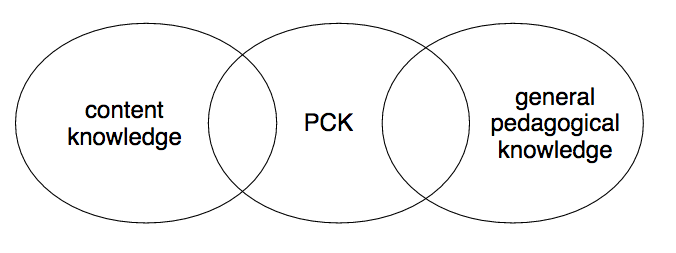
\includegraphics{../fig/pck.svg}
\caption{Pedagogical Content Knowledge}
\end{figure}

This training course focuses on general pedagogical knowledge through
the two major categories (educational psychology and instructional
design) described above. It assumes you know as much as you need to
about basic programming (our content knowledge).

When it comes to PCK, we will see later \secref{sec:practices} some
of the PCK of the Software and Data Carpentry communities at
work. Within Software Carpentry, we are also trying to support the
curation of PCK by including an instructor's guide with each lesson
that describes particular teaching techniques for that lesson's
content.

Finally, this training includes times for discussion, observation, and
feedback, precisely so that participants are able to share their PCK
with each other over the course of the next two days.

\begin{callout}{Examples of PCK}{callout:examples-of-pck}

\begin{itemize}
\item
  Gelman and Nolan's
  \emph{Teaching   Statistics: A Bag of Tricks} \cite{bib:gelman-nolan-stats-tricks}
  is full of PCK for teaching introductory statistics.
\item
  The \href{http://csteachingtips.org/}{CS Teaching Tips} site is
  gathering similar ideas for computing.
\end{itemize}
\end{callout}

\seclbl{Myths and Pseudoscience}{sec:myths-and-pseudoscience}

One
\href{https://en.wikipedia.org/wiki/Learning\_styles\#Learning\_modalities}{well-known
scheme} characterizes learners as visual, auditory, or kinesthetic
according to whether they like to see things, hear things, or do things.
This scheme is easy to understand, but as de Bruyckere and colleagues
point out in
\emph{Urban Myths About Learning and Education} \cite{bib:debruyckere-urban-myths},
it is almost certainly false.
Unfortunately, that hasn't stopped a large number of companies from
marketing products based on it to parents and school boards.

This is not the only myth to plague education. The learning pyramid that
shows we remember 10\% of what we read, 20\% of what we hear, and so on?
Myth.
The idea that ``brain games'' can improve our intelligence, or at least
slow its decline in old age?
Also a myth, as are the claims that the Internet is making us dumber or that
young people read less than they used to.

Computing education has its own myths. Mark Guzdial's
``Top 10 Myths About Teaching Computer Science'' \cite{bib:guzdial-top10} are:

The lack of women in Computer Science is just like all the other STEM
fields.

To get more women in CS, we need more female CS faculty.

A good CS teacher is a good lecturer.

Clickers and the like are an add-on for a good teacher.

Student evaluations are the best way to evaluate teaching.

Good teachers personalize education for students' learning styles.

High schools just can't teach CS well, so they shouldn't do it at all.

The real problem is to get more CS curriculum out into the hands of
teachers.

All I need to do to be a good CS teacher is model good software
development practice, because my job is to produce excellent software
engineers.

Some people are just born to program.

The last of these---the idea that there is a ``geek gene''---is as
pervasive as it is damaging. Elizabeth Patitsas and others have shown
that, contrary to a widely-held belief,
grades in computing classes are \emph{not} bimodal \cite{bib:patitsas-cs-grades},
i.e., there isn't one group that gets
it and another that doesn't. Many of the participants in our workshops
have advanced degrees in intellectually demanding subjects, but have
convinced themselves that they just don't have what it takes to be
programmers. If all we do is dispel that belief, we will have done them
a service.

\begin{callout}{Key Readings}{callout:key-readings}

An excellent overview of research results in education and learning is
Ambrose et al's
\emph{How Learning Works} \cite{bib:ambrose-hlw} (which is also an excellent example of what secondary
literature ought to look like).  Green's
\emph{Building a Better Teacher} \cite{bib:green-babt} is lighter but no less informative: it explores why
educational reforms in the past 50 years have mostly missed the mark,
and what we should be doing instead. The ultra-short summary
Deans for Impact report \cite{bib:deans-for-impact} contains useful, practical insights, and is
required reading for this training.

Pieces focusing specifically on computer science education include
Guzdial's
``Why Programming is Hard to Teach'' \cite{bib:guzdial-hard} and
``Top 10 Myths About Teaching Computer Science'' \cite{bib:guzdial-top10},
and Porter et al's ``Success in Introductory Programming: What Works?'' \cite{bib:porter-what-works},
all of which you should read before starting this class.
\end{callout}

\begin{discussion}{Three Kinds of Knowledge}{disc:three-kinds-of-knowledge}

Think of a memorable moment from a class you took or taught. Describe
it, and explain how the instructor used domain knowledge, general
pedagogical knowledge, and pedagogical content knowledge to create that
moment.
\end{discussion}

\begin{discussion}{Bottom Up or Top Down?}{disc:bottom-up-or-top-down}

How would you describe the way you learned what you already know about
using computers in research: bottom up, top down, or a mix of both? Is
that how you prefer to learn?
\end{discussion}

\chaplbl{Expertise and Memory}{s:memory}

Returning to educational psychology, we now discuss what distinguishes
expertise from earlier stages of learning, how expertise can be helpful
and harmful, and then describe concept maps, a tool that can help expose
expertise.

\seclbl{Connectivity}{sec:connectivity}

\secref{sec:novice} described
the key difference between novices and competent practitioners. What
makes experts different from either? The answer is not that they know
more facts: competent practitioners can memorize a lot of trivia without
any noticeable improvement to their performance.

To explain the difference, imagine for a moment that we store knowledge
as a graph in which facts are nodes and relationships are arcs. (This is
emphatically \emph{not} how our brains work, but it's a useful
metaphor.) The key difference between experts and people who are
``merely competent'' is that experts have many more connections, i.e.,
their mental models are much more densely connected.

To understand expert behavior, think about driving around a city,
comparing what it's like for the local and for the out-of-town driver.

This metaphor helps explain many observed aspects of expert behavior:

\begin{enumerate}
\item
  Experts can jump directly from a problem to its solution because there
  actually is a direct link between the two in their mind: where a
  competent practitioner would have to reason ``A, B, C, D, E'', the
  expert can go from A to E in a single step. We call this
  \emph{intuition}, and it isn't always a good thing: when asked to
  explain her reasoning, an expert often can't because she didn't
  actually go through any intermediate steps.

  \emph{In our example above, the local probably doesn't even think
  about which turns they're making on their way to the grocery store.
  They can drive on ``autopilot'' without really thinking. If someone
  asks them to go to a different location, they immediately know what
  they should do next to get to the right place.}
\item
  Experts are frequently so familiar with their subject that they can no
  longer imagine what it's like to \emph{not} see the world that way. As
  a result, they are often less good at teaching the subject than people
  with less expertise who still remember what it's like to have to learn
  the things. This is called \emph{expert blind spot}. It can be
  overcome with training, but it's part of why world-famous researchers
  are often poor lecturers.

  \emph{The local driver will forget to tell the out-of-towner that the
  bridge is under construction, or that there's always a train at 3:00,
  because it has been like that for years. The local driver will tell
  the out-of-towner to turn ``where the gas station used to be''.}
\item
  Densely-connected knowledge graphs also explains \emph{fluid
  representations}, e.g., expert mathematicians' ability to switch
  effortlessly between algebraic and geometric views of a problem.

  \emph{The local driver probably can use either the names of streets}
  or \emph{landmarks when giving directions. The out-of-towner only has
  street labels.}
\item
  Finally, this metaphor also explains why experts are better at
  diagnosis than competent practitioners: more linkages between facts
  makes it easier to reason backward from symptoms to causes. (And this
  in turn is why asking programmers to debug during job interviews gives
  a more accurate impression of their ability than asking them to
  program.)

  \emph{When the out-of-towner finally calls their local friend, saying
  ``well, we just passed Sycamore Street and we can see a restaurant
  named Nellie's Cafe'', the local can more easily figure out where the
  out-of-towner is, and how to get to their destination.}
\end{enumerate}

\begin{callout}{The J Word}{callout:the-j-word}

Experts often betray their blind spot by using the word ``just'' in
explanations, as in, ``Oh, it's easy, you just fire up a new virtual
machine and then you just install these four patches to Ubuntu and then
you just re-write your entire program in a pure functional style---no
problem.'' As we discuss later in \secref{sec:motivation},
the J word (also sometimes called the passive dismissive
adjective) is banned in our workshops, primarily because using it gives
learners the very clear signal that the instructor thinks their problem
is trivial and that they therefore must be stupid.
\end{callout}

The graph model of knowledge explains why helping learners make
connections is as important as introducing them to facts. The more
people you know in a group, the more likely you are to remain part of
that group. Similarly, the more connections a fact has to other facts,
the more likely the fact is to be remembered. This builds on our earlier
idea of mental models - a mental model is a way to facilitate making
connections between separate facts.

\begin{callout}{Repetition vs.~Reflective Practice}{callout:repetition-vs.reflective-practice}

The idea that ten thousand hours of practice will make someone an expert
in some field is widely known, but reality is much more complex. First,
practice is not doing the same thing over and over again: practice is
doing similar but subtly different things, getting feedback, and then
changing behavior in response to that feedback to get cumulatively
better. Doing the same thing over and over again is much more likely to
solidify bad habits than perfect performance.

Second, a \href{http://pss.sagepub.com/content/25/8/1608}{meta-study in
2014} found that ``\ldots{}deliberate practice explained 26\% of the
variance in performance for games, 21\% for music, 18\% for sports, 4\%
for education, and less than 1\% for professions.'' One explanation for
this variation is that deliberate practice works best when the rules for
evaluating success are very stable, but is less effective when there are
more factors at play.
\end{callout}

\seclbl{Concept Maps}{sec:concept-maps}

Our tool of choice to represent an expert's knowledge graph is the
\emph{concept map}. A concept map is simply a picture of someone's
mental model of a domain: facts are bubbles, and connections are
labelled arcs. It is important that they are labelled: saying ``X and Y
are related'' is only helpful if we explain what the relationship
\emph{is}. And yes, one person's fact may be another person's
connection, but by \emph{externalizing cognition} (i.e., making thought
processes and mental models visible), concept maps help spark and focus
discussion.

\begin{callout}{There's More Than One Way to Do It}{callout:theres-more-than-one-way-to-do-it}

Concept maps are just one way to represent our understanding of a
subject. Flowcharts, decision trees, and blueprints can be even more
useful in some contexts. For example,
\href{fixme-abela}{this diagram}
(taken from \href{http://extremepresentation.typepad.com/blog/2006/09/choosing\_a\_good.html}{a blog post}
by Andrew Abela) is an excellent way to organize and present
an understanding of how to choose the right kinds of chart for
displaying different kinds of data.
\end{callout}

To show what concept maps look like, consider this simple \texttt{for}
loop in Python:

\begin{verbatim}
for ch in "abc":
    print(2*ch)
\end{verbatim}

\{: .source\}

The three key concepts used in this loop are:

\begin{figure}[htbp]
\centering
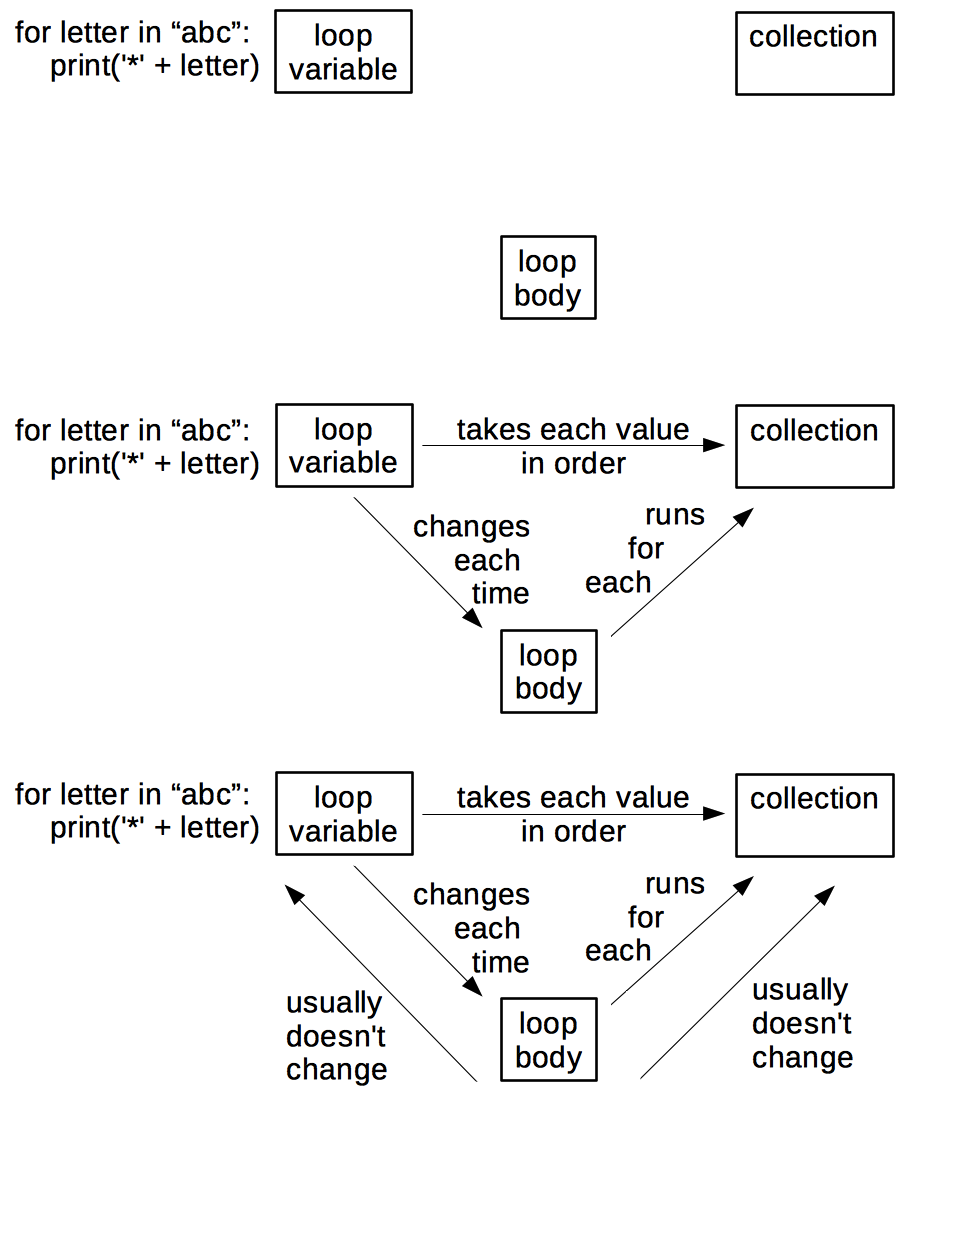
\includegraphics{../fig/for-loop-concepts.png}
\caption{Key Concepts}
\end{figure}

(In this case it's easy to connect the concepts to concrete elements in
the program, but that may not always be the case.) The key
relationships, which are as important as the concepts themselves, are:

\begin{figure}[htbp]
\centering
\includegraphics{../fig/for-loop-arcs.png}
\caption{Relationships}
\end{figure}

A quick count shows that there are actually 6 things here, not just 3,
so we're already brushing up against the limits of short-term memory. If
we add two more facts to show things that are usually (but not always)
true:

\begin{figure}[htbp]
\centering
\includegraphics{../fig/for-loop-rec.png}
\caption{Recommendations}
\end{figure}

the count rises to 8, which is a good size for a single teaching
episode. A few other concept maps drawn by previous participants in this
training course are listed below:

\begin{itemize}
\item
  \href{../fig/array-math.png}{Array Math}
\item
  \href{../fig/conditionals.png}{Conditionals}
\item
  \href{../fig/create-destroy.png}{Creating and Destroying Files}
\item
  \href{../fig/dict-set.png}{Sets and Dictionaries in Python}
\item
  \href{../fig/io.png}{Input and Output}
\item
  \href{../fig/lists-loops.png}{Lists and Loops}
\end{itemize}

Most of these are larger than our recommended limit, but that's not
necessarily a bad thing: after drawing a concept map for an entire
subject, a lesson designer can then carve out tightly-connected
sub-graphs to make individual episodes.

Concept maps can be used in many ways:

\begin{enumerate}
\item
  To aid solo design of a lesson by helping authors figure out what
  they're trying to teach. Crucially, a concept map separates content
  from order: in our experience, people rarely wind up teaching things
  in the order in which they first drew them.
\item
  They aid communication with fellow lesson designers. Instructors with
  very different ideas of what they're trying to teach are likely to
  pull their learners in different directions. Drawing and sharing
  concept maps isn't guaranteed to prevent this, but it certainly helps.
\item
  Concept maps also aid communication with learners. While it's possible
  to give learners a pre-drawn map at the start of a lesson for them to
  annotate, it's better to draw it piece by piece while teaching to
  reinforce the ties between what's in the map and what the instructor
  said. (We will return to this idea below when discussing Mayer's work
  on multimedia learning.)
\item
  Concept maps are also a useful formative assessment technique: having
  learners draw concept maps of what they think they just heard shows
  the instructor what was missed and what was mis-understood. Reviewing
  the learners' concept maps is too time-consuming for use in workshops,
  but very useful in weekly lectures \emph{once learners are familiar
  with the technique}: as
  \href{http://www.amazon.com/Facts-Fallacies-Software-Engineering-Robert/dp/0321117425/}{Glass
  observed}, any new tool or technique initially slows people down.
\end{enumerate}

Concept maps are also useful for many other kinds of tasks. For example,
the next time you have a team meeting, give everyone a sheet of paper
and have them spend a few minutes drawing a concept map of the project
you're all working on---separately. On the count of three, have everyone
reveal their concept maps simultaneously. The discussion that follows
everyone's realization of how different their mental models of the
project's aims and organization are is always interesting\ldots{}

Concept maps are also a useful way to organize one's thoughts before
putting together a talk or writing a paper. As with lessons, they allow
us to \emph{externalize cognition}, i.e., to get our thoughts out where
we can see them (and see the contradictions that have happily been
swimming around inside our heads without bumping into each other).

\begin{challenge}{Concept Mapping}{chal:concept-mapping}

Create a hand drawn concept map for something you would teach in five
minutes. (Possibly for the same subject that you used to create a
multiple choice question before.) Trade with a partner, and critique
each other's maps. Do they present concepts or surface detail? Which of
the relationships in your partner's map do you consider concepts and
vice versa?
\end{challenge}

\begin{callout}{Building Concept Maps Together}{callout:building-concept-maps-together}

Concept maps can be used as a classroom discussion exercise. Put
learners in small groups (2-4 people each), give each group some sticky
notes on which a few key concepts are written, and have them build a
concept map on a whiteboard by placing those sticky notes, connecting
them with labelled arcs, and adding any other concepts they think they
need.
\end{callout}

\begin{callout}{What Are We Doing Again?}{callout:what-are-we-doing-again}

Concept maps can also be used to help build a shared understanding of
what a project is trying to accomplish. Everyone independently draws a
concept map to show what they think the project's goals and constraints
are. Those concept maps are then revealed simultaneously. The ensuing
discussion can be\ldots{}vigorous.
\end{callout}

\seclbl{Seven Plus or Minus Two}{sec:seven-plus-or-minus-two}

\begin{challenge}{The Serial Position Effect}{chal:the-serial-position-effect}

Read the following list and try to memorize the items in it:

cat, apple, ball, tree, square, head, house, door, box, car, king,
hammer, milk, fish, book, tape, arrow, flower, key, shoe

Without looking at the list again, write down as many words from the
list as you can. Compare to other members of the group. What words are
remembered the most?

\href{http://cat.xula.edu/thinker/memory/working/serial}{This website}
implements an interactive version of this exercise.
\end{challenge}

While the graph model of knowledge is inaccurate but useful, another
simple model of knowledge has a sound physical basis. As a rough
approximation, human memory can be divided into two different storage
layers. The first is called \emph{long-term} or \emph{persistent
memory}. It is where we store things like our password, our home
address, and what the clown did at our eighth birthday party that scared
us so much. It is essentially unbounded (barring injury or disease, we
will die before it fills up) but it is slow to access---too slow to help
us handle hungry lions and disgruntled family members.

Evolution has therefore given us a second system called
\emph{short-term} or \emph{working memory}. It is much faster, but also
much smaller: in 1956, Miller estimated that the average adult's working
memory could hold
\href{https://en.wikipedia.org/wiki/The\_Magical\_Number\_Seven,\_Plus\_or\_Minus\_Two}{7±2
items} for a few seconds before things started to drop out. This is why
phone numbers are typically 7 or 8 digits long: back when phones had
dials instead of keypads, that was the longest string of numbers most
adults could remember accurately for as long as it took the dial to go
around and around. It's also why sports teams tend to have about half a
dozen members, or be broken down into smaller groups (such as the
forwards and backs in rugby).

When we memorize words in a list and are asked to immediately recall
them, the words first presented will have the best chance to be
transferred into long-term memory. On the other hand, the items that are
presented last might still be in short-term memory. These are referred
to as the primacy and recency effects, respectively, and they together
form the
\href{https://en.wikipedia.org/wiki/Serial\_position\_effect}{memory
serial position effect}.

\begin{callout}{Chunking}{callout:chunking}

Our minds can store larger numbers of facts in short-term memory by
creating \emph{chunks}. For example, most of us will remember a word we
read as a single item, rather than as a sequence of letters. Similarly,
the pattern made by five spots on cards or dice is remembered as a whole
rather than as five separate pieces of information. Chunks allow us to
manage larger problems, but can also mislead us if we mis-identify
something, i.e., see it as something it isn't.
\end{callout}

7±2 is probably the most important number in programming. When someone
is trying to write the next line of a program, or understand what's
already there, she needs to keep a bunch of arbitrary facts straight in
her head: what does this variable represent, what value does it
currently hold, etc. If the number of facts grows too large, her mental
model of the program comes crashing down (something we have all
experienced).

7±2 is also the most important number in teaching. An instructor cannot
push information directly into a learner's long-term memory. Instead,
whatever she presents is first represented in the learner's short-term
memory, and is only transferred to long-term memory after it has been
held there and rehearsed. If we present too much information too
quickly, the new will displace the old before it has a chance to
consolidate in long-term memory.

This is why it's very important to use a technique like concept mapping
a lesson before teaching it - an instructor needs to identify just how
many pieces of separate information will need to be ``stored'' in memory
as part of the lesson.

\begin{quote}
Do concept maps feel useful to you? Are there other ways of drawing
knowledge that appeal to you more?
\end{quote}

\chaplbl{Cognitive Load}{s:load}

In our final topic in educational psychology, we'll be learning more
about human memory: specifically how to remove unnecessary ``load'' in
order to facilitate learning.

\seclbl{Battling Theories}{sec:battling-theories}

In 2006, Kirschner, Sweller, and Clark published a paper titled
``\href{http://www.cogtech.usc.edu/publications/kirschner\_Sweller\_Clark.pdf}{Why
Minimal Guidance During Instruction Does Not Work: An Analysis of the
Failure of Constructivist, Discovery, Problem-Based, Experiential, and
Inquiry-Based Teaching}''. In the abstract, they say:

\begin{quote}
Although unguided or minimally guided instructional approaches are very
popular and intuitively appealing\ldots{}these approaches ignore both
the structures that constitute human cognitive architecture and evidence
from empirical studies over the past half-century that consistently
indicate that minimally guided instruction is less effective and less
efficient than instructional approaches that place a strong emphasis on
guidance of the student learning process. The advantage of guidance
begins to recede only when learners have sufficiently high prior
knowledge to provide ``internal'' guidance.
\end{quote}

The paper set off a minor academic firestorm, because beneath the jargon
the authors were claiming that
\href{https://en.wikipedia.org/wiki/Inquiry-based\_learning}{inquiry-based
learning}---allowing learners to ask their own questions, set their own
goals, and find their own path through a subject---doesn't actually work
very well. Kirschner et al's argument was that it requires learners to
simultaneously master a domain's factual content and its search and
problem-solving strategies. Fostering creativity and independence is
intuitively appealing, but that doesn't mean it works.

One of the paper's authors (Sweller) proposed an alternative based on
the theory of
\emph{\href{https://en.wikipedia.org/wiki/Cognitive\_load}{cognitive
load}}. It posits that people have to deal with three things when
they're learning:

\begin{itemize}
\item
  \emph{Intrinsic} load is what they have to keep in mind in order to
  carry out a learning task.
\item
  \emph{Germane} load is the (desirable) mental effort required to
  create linkages between new information and old (which is one of the
  things that distinguishes learning from memorization).
\item
  \emph{Extraneous} load is everything else that distracts or gets in
  the way.
\end{itemize}

Cognitive load theory's proponents claim that eliminating extraneous
cognitive load accelerates learning. Unsurprisingly, it too has
\href{https://edtechdev.wordpress.com/2009/11/16/cognitive-load-theory-failure/}{been
criticized}, most particularly for being unfalsifiable. Critics of
cognitive load theory say that since there's no way to tell in advance
of an experiment whether something is germane or not, any result can be
justified after the fact by labelling things that hurt performance as
``extraneous'' and things that don't ``germane''.

However, some predictions \emph{can} be made. One example is work by
Mayer and colleagues on the
\emph{\href{https://en.wikipedia.org/wiki/Split\_attention\_effect}{split-attention
effect}}. Linguistic and visual input are processed by different parts
of the human brain, and linguistic and visual memories are stored
separately as well. This means that correlating linguistic, auditory,
and visual streams of information takes cognitive effort: when someone
reads something while hearing it spoken aloud, their brain can't help
but check that it's getting the same information on both channels.
Learning is therefore more effective when redundant information is
\emph{not} being presented simultaneously in two different channels. For
example, people find it harder to learn from a video that has both
narration and on-screen captions than from one that has either the
narration or the captions but not both.

\seclbl{Faded Examples}{sec:faded-examples}

According to cognitive load theory, searching for a solution strategy is
an extra burden on top of applying that strategy. We can therefore
accelerate learning by giving learners worked examples that show them a
problem and a detailed step-by-step solution, followed by a series of
\emph{faded examples}. The first of these presents a nearly-complete use
of the same problem-solving strategy just demonstrated with a small
number of blanks for the learner to fill in. The next problem is also of
the same type, but has more blanks, and so on until the learner is asked
to solve the entire problem.

Faded examples work because they introduce the problem-solving strategy
piece by piece. At each step, learners have one new problem to tackle.
This is less intimidating than a blank screen or a blank sheet of paper.
It also encourages learners to think about the similarities and
differences between various approaches, which helps create the linkages
in the mental model that instructors want them to form.

For example, someone teaching Python might start by explaining this:

\begin{verbatim}
# total_length(["red", "green", "blue"]) => 12
def total_length(words):
    total = 0
    for word in words:
        total += len(word)
    return total
\end{verbatim}

\{: .source\}

then ask learners to fill in the blanks in:

\begin{verbatim}
# word_lengths(["red", "green", "blue"]) => [3, 5, 4]
def word_lengths(words):
    lengths = ____
    for word in words:
        lengths ____
    return lengths
\end{verbatim}

\{: .source\}

The next problem might be:

\begin{verbatim}
# concatenate_all(["red", "green", "blue"]) => "redgreenblue"
def concatenate_all(words):
    result = ____
    for ____ in ____:
        ____
    return result
\end{verbatim}

\{: .source\}

and learners would finally be asked to tackle:

\begin{verbatim}
# acronymize(["red", "green", "blue"]) => "RGB"
def acronymize(words):
    ____
\end{verbatim}

The key to constructing a good faded example is to think about the
problem-solving strategy or solution pattern that it is meant to teach.
For example, the series of problems above illustrate the
\emph{accumulator pattern}, in which the results of processing items
from a collection are repeatedly added to a single variable in some way
to create the final result.

\begin{challenge}{Create a Faded Example from a Lesson}{chal:create-a-faded-example-from-a-lesson}

The following exercise should be done in groups of 2-3.

\begin{enumerate}
\item
  Pick a block of code from an existing Software or Data Carpentry
  lesson, or from another lesson you have taught recently.
\item
  Replace 2-3 pieces of the code with a blank.
\item
  Write a question to test the student's ability to correctly fill in
  that blank.
\item
  Paste your faded example in the Etherpad.
\end{enumerate}
\end{challenge}

\seclbl{Parsons Problems}{sec:parsons-problems}

Another kind of exercise designed to reduce cognitive load is a
\emph{Parsons Problem}, in which learners are presented with the jumbled
parts of a solution and asked to put them in order. When learning a
language, for example, students could be asked to order a set of words
to create a grammatically correct response to a question. Similarly, our
learners can be given the lines of code needed to solve a problem and
asked to arrange them. Learners can then be told that they have all the
lines they need save one, and so on.

Here is a really nice online Parsons Problem interactive tool.
\href{http://runestoneinteractive.org/LearningAtScale/parsons.html}{Try
it out!}

\begin{challenge}{Parsons Problems}{chal:parsons-problems}

Write 5 or 6 lines of code that does something useful, jumble them, then
add one more line that looks plausible but isn't needed to solve the
problem. How well can your partner tell which line is unnecessary?
\end{challenge}

\chaplbl{Lessons}{s:lessons}

So far, we've spent a lot of time talking about details of teaching and
learning.
Yesterday we talked about specific teaching tools and how
people learn; today we've talked about Software Carpentry and Data
Carpentry teaching more specifically.
So to wrap up the training, we're
going to go back and look a bit more at lessons - the actual content
that you will be preparing and teaching as a Software/Data Carpentry
instructor. This will two forms: we'll talk about lesson design
generally, and about the Software and Data Carpentry lessons in
particular.

\seclbl{Writing Lessons}{sec:writing-lessons}

A theme you may have noticed in our material so far is a need to start
``at the end''. To write a multiple-choice question, you have to start
with
misconceptions and work backward to write a question to diagnose
them. To write a faded example, you start with the full example and
remove pieces. So here, the way to write a lesson is not to just sit
down and start writing. The most important thing is to know your
audience and what you want them to learn, and then to develop your
lesson accordingly.

\seclbl{Learner Profiles}{sec:learner-profiles}

The first piece - your audience, can be identified in many ways.
Frequently people who are hosting a workshop have a specific audience in
mind, based on their own experience.

One ``creative'' way to characterize the audience for a course is to
write \emph{learner profiles}. This technique is borrowed from user
interface design, where short profiles of typical users are created to
help designers think about their audience's needs, and to give them a
shorthand for talking about specific cases.

Learner profiles have three parts: the person's general background, the
problem they face, and how the course will help them. A learner profile
for Software Carpentry might be:

\begin{quote}
João is an agricultural engineer doing his masters in soil physics. His
programming experience is a first year programming course using C. He
was never able to use this low-level programming into his activities,
and never programmed after the first year.

His work consists of evaluating physical properties of soil samples from
different conditions. Some of the soil properties are measured by an
automated device that sends logs in a text format to his machine. João
has to open each file in Excel, crop the first and last quarters of
points, and calculate an average.

Software Carpentry will show João how to write shell scripts to count
the lines and crop the right range for each file, and how to use R to
read these files and calculate the required statistics. It will also
show him how to put his programs and files under version control so that
he can re-run analyses and figure out which results may have been
affected by changes.
\end{quote}

\begin{challenge}{Learner Profiles}{chal:learner-profiles}

Read \href{http://software-carpentry.org/audience/}{Software Carpentry's
learner profiles} and then write one that describes a fictional
colleague of your own. Who are they, what problems do they face, and how
will this training help them? Try to be as specific as possible.
\end{challenge}

\seclbl{Writing Learning Objectives}{sec:writing-learning-objectives}

Summative and formative assessments help instructors figure out what
they're going to teach, but in order to communicate that to learners and
other instructors, we should also write \emph{learning objectives}. A
learning objective is a single sentence describing what a learner will
be able to do once they have sat through the lesson, in order to
demonstrate ``learning.'' That requires thinking critically about what
exactly you want people to learn.

It's dangerously easy to come up with fuzzy learning objectives. A broad
statement like ``Understand git'' could mean many different specific
goals, like:

\begin{itemize}
\item
  Learners can revert a change to a file using git.
\item
  Learners will name three benefits of using a version control system
  like git.
\item
  Learners will compare the collaboration features of git and dropbox.
\end{itemize}

What we want are specific, verifiable descriptions of what learners can
do to demonstrate their learning. Each learning objective should have
\emph{a measurable or verifiable verb} specifying what the learner will
do, and should specify the \emph{criteria for acceptable performance}.

Writing these kinds of learning objectives may seem restrictive or
limiting, but will make both you and your learners happier in the long
run. You will end up with clear guidelines for both your teaching and
assessment, and your learners will appreciate the clear expectations.

In order to formulate good learning objectives we need to decide what
kinds of learning we are aiming for. There is a difference between
knowing the atomic weight of fluorine and understanding what elements
it's likely to bond with and why. Similarly, there's a difference
between being able to figure out why a microscope isn't focusing
properly and being able to design a new microscope that focuses more
easily. What we need is a taxonomy of understanding that is
hierarchical, measurable, stable, and cross-cultural.

The best-known attempt to build one is
\href{https://en.wikipedia.org/wiki/Bloom's\_taxonomy}{Bloom's taxonomy},
which was first published in 1956. More recent efforts are Wiggins and
McTighe's \emph{facets of understanding} and Fink's taxonomy from his
book
\emph{\href{http://www.amazon.com/Creating-Significant-Learning-Experiences-Integrated/dp/1118124251/}{Creating
Significant Learning Experiences}}. The table below compares them and
shows some of the verbs typically used in learning objectives written
for each level.

\begin{verbatim}
<th>Bloom's taxonomy</th>
<th>Facets of understanding (Wiggins & McTighe)</th>
<th>Taxonomy of significant learning (Fisk)</th>
<th>Typical learning objective verbs</th>
\end{verbatim}

\begin{verbatim}
<td>
  <strong>Knowledge</strong>: recalling learned information
</td>
<td>
  <strong>Explain</strong>: provide sophisticated and apt explanations and theories that provide knowledgeable and justified accounts of phenomena, facts, and data
</td>
<td>
  <strong>Foundational knowledge</strong>: the facts, terms, formulas, concepts, principles, etc. that one understands and remembers
</td>
<td>
  name, define, recall
</td>
\end{verbatim}

\begin{verbatim}
<td>
  <strong>Comprehension</strong>: explaining the meaning of information
</td>
<td>
  <strong>Interpret</strong>: interpretations, narratives, and translations that provide meaning; make subjects personal or accessible through images, anecdotes, analogies, and models
</td>
<td>
  <strong>Application</strong>: using critical, creative, and practical (decision-making, problem-solving) skills
</td>
<td>
  restate, locate, explain, recognize
</td>
\end{verbatim}

\begin{verbatim}
<td>
  <strong>Application</strong>: applying what one knows to novel, concrete situations
</td>
<td>
  <strong>Apply</strong>: ability to use and adapt what one knows to new situations and in various contexts
</td>
<td>
  <strong>Integration</strong>: making connections among ideas, subjects, and people
</td>
<td>
  apply, demonstrate, use
</td>
\end{verbatim}

\begin{verbatim}
<td>
  <strong>Analysis</strong>: breaking down a whole into its component parts and explaining how each part contributes to the whole
</td>
<td>
  <strong>Have perspective</strong>: critical and insightful points of view; see the big picture
</td>
<td>
  <strong>Human dimensions</strong>: learning about and changing one's self; interacting with others
</td>
<td>
  differentiate, criticize, compare
</td>
\end{verbatim}

\begin{verbatim}
<td>
  <strong>Synthesis</strong>: assembling components to form a new and integrated whole
</td>
<td>
  <strong>Empathize</strong>: ability to get inside another's feelings and perspectives; use prior indirect experience to perceive sensitively
</td>
<td>
  <strong>Caring</strong>: identifying and changing one's feelings, values, and interests
</td>
<td>
  design, construct, organize
</td>
\end{verbatim}

\begin{verbatim}
<td>
  <strong>Evaluation</strong>: using evidence to make judgments about the relative merits of ideas and materials
</td>
<td>
  <strong>Have self-knowledge</strong>: perceive how one's patterns or thought and action shape and impede one's own understanding
</td>
<td>
  <strong>Learning how to learn</strong>: becoming a better, self-directed learner; learning to ask and answer questions
</td>
<td>
  choose, rate, select
</td>
\end{verbatim}

\begin{verbatim}
<td colspan="3">
  Reproduced with additions from <a href="http://www.lifescied.org/content/6/2/85.full">Allen and Tanner</a>'s
  "Putting the Horse Back in Front of the Cart: Using Visions and Decisions about High-Quality Learning Experiences to Drive Course Design" (2007)
</td>
\end{verbatim}

Here is an example of a successively-improved lesson objective:

\begin{itemize}
\item
  \textit{Learner will be given opportunities to learn good programming practices.}
  \\
  Describes the lesson's content, not the attributes of successful students.
\item
  \textit{Learner will have a better appreciation for good programming practices.}
  \\
  Doesn't start with an active verb or define the level of learning,
  and the subject of learning has no context and is not specific.
\item
  \textit{Learner will understand principles of good programming.}
  \\
  Starts with an active verb, but doesn't define the level of learning,
  and the subject of learning is still too vague for assessment.
\item
  \textit{Learner will write one-page data analysis scripts for research purposes using R Studio.}
  \\
  Starts with an active verb, defines the level of learning,
  and provides context to ensure that outcomes can be assessed.
\end{itemize}

Baume's guide to
writing and using good learning outcomes \cite{bib:baume-fixme} is a good longer discussion of these
issues.

\begin{challenge}{Evaluate SWC and DC Learning Objectives}{chal:evaluate-swc-and-dc-learning-objectives}

Your instructor has posted links to a handful of current Software and
Data Carpentry lessons in the Etherpad. Take a minute to select one
learning objective from one of those lessons, then complete the
following steps to evaluate it and reword it to make it sharper.

\begin{enumerate}
\item
  Identify the learning objective verb.
\item
  Decide what type of learning outcome this applies to
  (i.e.~comprehension, application, evaluation).
\item
  Reword the learning objective for a different learning outcome (e.g.,
  from application to knowledge based outcome or vice versa).
\item
  Pair up to discuss your rewording or help each other with point 3 or 4
  if necessary.
\item
  Share the original and your re-worded learning objectives in the Etherpad.
\end{enumerate}
\end{challenge}

\seclbl{Reverse Instructional Design}{sec:reverse-instructional-design}

Most people design courses as follows:

\begin{enumerate}
\item
  The chair tells you that you have to teach something you haven't
  thought about in ten years.
\item
  You start writing slides to explain what you know about the subject.
\item
  After two or three weeks, you make up an assignment based more or less
  on what you've taught so far.
\item
  You repeat step 3 several times.
\item
  You stay up 'til the wee hours to make up a final exam.
\end{enumerate}

There's a better way, and to explain it, we first need to explain how
\emph{\href{https://en.wikipedia.org/wiki/Test-driven\_development}{test-driven
development}} (TDD) is used in software development. When programmers
are using TDD, they don't write software and then (possibly) write
tests. Instead, they write the tests first, then write just enough new
software to make those tests pass, and then clean up a bit.

TDD works because writing tests forces programmers to specify exactly
what they're trying to accomplish and what ``done'' looks like. It's
easy to be vague when using a human language like English or Korean;
it's much harder to be vague in Python or R.

TDD also reduces the risk of endless polishing, and increases the
likelihood that tests will actually get written. (Somehow, people always
seem to run out of time\ldots{}) Finally, writing the tests first
reduces the risk of confirmation bias: someone who hasn't written a
program is much more likely to be objective when testing it than its
original author.

A similar ``backward'' method works very well for lesson design. As
described in Wiggins and McTighe's
\emph{\href{http://www.amazon.com/Understanding-Design-Expanded-Grant-Wiggins/dp/0131950843/}{Understanding
by Design}}, the method proceeds through four stages:

\begin{enumerate}
\item
  Identify what is worth learning (e.g., draw concept maps).
\item
  Decide what constitutes evidence that learning has taken place (i.e.,
  create the final exam or some other summative assessment).
\item
  Design practice work to prepare learners for what they will have to do
  during the summative assessment. These should include formative
  assessments to be done in class and the exercises to be done out of
  class.
\item
  Sort those practices in order of increasing complexity and then write
  short episodes to close the gap between what learners know and what
  they need to know in order to do each one. (An actual classroom lesson
  will then consist of several such episodes, each building toward a
  quick formative assessment.)
\end{enumerate}

This \emph{reverse instructional design} method helps keep teaching
focused on its objectives. It also ensures that learners don't face
anything on the final exam that the course hasn't prepared them for.

\begin{callout}{How and Why to Fake It}{callout:how-and-why-to-fake-it}

One of the most influential papers in the history of software
engineering was Parnas and Clements'
``\href{http://dx.doi.org/10.1109/TSE.1986.6312940}{A Rational Design
Process: How and Why to Fake It}''
(\href{http://www.ics.uci.edu/~taylor/classes/121/IEEE86\_Parnas\_Clement.pdf}{PDF}),
in which they pointed out that in real life we move back and forth
between gathering requirements, interface design, programming, and
testing, but when we write up our work it's important to describe it as
if we did these steps one after another so that other people can retrace
our steps. The same is true of lesson design: while we may change our
mind about what we want to teach based on something that occurs to us
while we're writing an MCQ, we want the notes we leave behind to present
things in the order described above.
\end{callout}

\begin{discussion}{Teaching to the Test}{discuss:teaching-to-the-test}

Is reverse instructional design ``teaching to the test''? I.e., does it
steer teachers toward getting their students to pass an exam rather than
learn things?

Reverse instructional design is \emph{not} the same thing as ``teaching
to the test''. When using RID, teachers set goals to aid in lesson
design, and may never actually give the final exam that they wrote. In
many school systems, on the other hand, an external authority defines
assessment criteria for all learners, regardless of their individual
situations, and the outcomes of those summative assessments directly
affect the teachers' pay and promotion. Green's
\emph{\href{http://www.amazon.com/Building-Better-Teacher-Teaching-Everyone/dp/0393351084/}{Building
a Better Teacher}} argues that this focus on measurement is appealing to
those with the power to set the tests, but is unlikely to improve
outcomes unless it is coupled with support for teachers to make
improvements based on test outcomes. This is often missing, because as
Scott pointed out in
\emph{\href{http://www.amazon.com/Seeing-like-State-Certain-Condition/dp/0300078153/}{Seeing
Like a State}}, large organizations usually value uniformity over
productivity. \{: .solution\}
\end{discussion}

\begin{callout}{The Minimal Manual}{callout:the-minimal-manual}

Carroll et al's 1987 paper
``The Minimal Manual'' \cite{bib:carroll-minimal-manual}
outlines an approach to documentation and instruction
in which each lesson is one page long and describes how to accomplish
one concrete task. Its focus on immediate application, error recognition
and recovery, and reference use after training makes it an interesting
model for Software and Data Carpentry.
\end{callout}

\seclbl{Software and Data Carpentry Lessons}{sec:software-and-data-carpentry-lessons}

It would be nice to say that the Software and Data Carpentry lessons
were all developed using perfect reverse instructional design. While
that's not necessarily true, all of the lessons are constantly being
revised and edited with certain core objectives in mind.

The main aim of the Unix shell lesson is to familiarize people with a
handful of basic concepts that crop up in many other areas of computing:

\begin{itemize}
\item
  the notions of a path and a home directory
\item
  the use of history and tab completion to save time (and prevent
  mistakes)
\item
  manipulating text using \texttt{head}, \texttt{tail}, \texttt{grep},
  and related tools
\item
  combining existing tools using pipes instead of writing new ones
\item
  using loops to repeat operations
\end{itemize}

The aims of the version control lesson are to teach people:

\begin{itemize}
\item
  how to keep track of their work,
\item
  how to collaborate with other people online, and
\item
  enough about privacy and licensing that they can begin to make
  sensible decisions about what to put where and how to share it.
\end{itemize}

The ostensible aim of the programming lessons are to show people how to
build modular programs out of small functions that can be read, tested,
and re-used. However, these concepts turn out to be hard to convey to
people who are still learning the syntax of a programming language
(forest and trees), so in practice the programming lessons focus
primarily on the mechanics of doing common operations in those
languages.

\seclbl{Data Carpentry}{sec:data-carpentry}

Data Carpentry's \href{http://datacarpentry.org/lessons/}{lessons}
are domain-specific and cover data organization, manipulation, and
visualization skills relevant to the target domain. These goals include:

\begin{itemize}
\item
  \href{http://datacarpentry.org/lessons/\#ecology-workshop}{Ecology}

  \begin{itemize}
    \item
    Focuses on general data management skills (proper data formatting
    and tracking) and tools for manipulating and visualizing tabular
    data.
  \end{itemize}
\item
  \href{http://datacarpentry.org/lessons/\#genomics-workshop}{Genomics}

  \begin{itemize}
    \item
    Specialized for researchers with sequence data, includes specific
    bioinformatics tools and how to use large-scale computing
    resources.
  \end{itemize}
\item
  \href{http://datacarpentry.org/lessons/\#geospatial-data-workshop}{Geospatial
  Data}
\end{itemize}

There are also materials in development and testing for:

\begin{itemize}
\item
  \href{http://datacarpentry.org/lessons/\#social-science-materials}{Social
  Science}
\item
  and \href{http://datacarpentry.org/semester-biology/}{a
  semester-long Biology course}.
\end{itemize}

Other Data Carpentry lessons are in the incubator stage.

\begin{quote}
How practical do you think it would be to use the techniques you've
learned in this workshop in regular teaching? In particular, do you
think you would have enough time to prepare and teach lessons the ways
you have been shown?
\end{quote}


\part{Teaching}

\chaplbl{Teaching as a Performance Art}{sec:performance}

Continuing with our theme of instructor-as-performer, let's discuss some
research that suggests that improvement in educational outcomes must be
driven by practice and communities of practice. The tricks and
techniques that make teaching effective cannot be mandated from above,
but will develop into widespread effectiveness only as they are shared
through a community of teaching practice.

\seclbl{Lesson Study}{sec:lesson-study}

Many people assume that teachers are born, not made. From politicians to
researchers and teachers themselves, most reformers have designed
systems to find and promote those who can teach and eliminate those who
can't. As Elizabeth Green describes in
\emph{Building a Better Teacher} \cite{bib:green-babt}, though,
that assumption is wrong, which is why
educational reforms based on it have repeatedly failed.

The book is written as a history of the people who have put that puzzle
together in the US. Its core begins with a discussion of what James
Stigler discovered during a visit to Japan in the early 1990s:

\begin{quote}
Some American teachers called their pattern ``I, We, You'': After
checking homework, teachers announced the day's topic, demonstrating a
new procedure (I)\ldots{} Then they led the class in trying out a sample
problem together (We)\ldots{} Finally, they let students work through
similar problems on their own, usually by silently making their way
through a worksheet (You)\ldots{}

The Japanese teachers, meanwhile, turned ``I, We, You'' inside out. You
might call their version ``You, Y'all, We.'' They began not with an
introduction, but a single problem that students spent ten or twenty
minutes working through alone (You)\ldots{} While the students worked,
the teacher wove through the students' desks, studying what they came up
with and taking notes to remember who had which idea. Sometimes the
teacher then deployed the students to discuss the problem in small
groups (Y'all). Next, the teacher brought them back to the whole group,
asking students to present their different ideas for how to solve the
problem on the chalkboard\ldots{} Finally, the teacher led a discussion,
guiding students to a shared conclusion (We).
\end{quote}

It's tempting but wrong to think that this particular teaching technique
is Japan's secret sauce. The actual key is revealed in the description
of Akihiko Takahashi's work. In 1991, he visited the United States in a
vain attempt to find the classrooms described a decade earlier in a
report by the National Council of Teachers of Mathematics. He couldn't
find them. Instead, he found that American teachers met once a year (if
that) to exchange ideas about teaching, compared to the weekly or even
daily meetings he was used to. What was worse:

\begin{quote}
The teachers described lessons they gave and things students said, but
they did not \emph{see} the practices. When it came to observing actual
lessons---watching each other teach---they simply had no
opportunity\ldots{} They had, he realized, no \emph{jugyokenkyu}.
Translated literally as ``lesson study'', \emph{jugyokenkyu} is a bucket
of practices that Japanese teachers use to hone their craft, from
observing each other at work to discussing the lesson afterward to
studying curriculum materials with colleagues. The practice is so
pervasive in Japanese schools that it is\ldots{}effectively invisible.

And here lay the answer to {[}Akihiko's{]} puzzle. Of course the
American teachers' work fell short of the model set by their best
thinkers\ldots{} Without \emph{jugyokenkyu}, his own classes would have
been equally drab. Without \emph{jugyokenkyu}, how could you even teach?
\end{quote}

So what does \emph{jugyokenkyu} look like in practice?

\begin{quote}
In order to graduate, education majors not only had to watch their
assigned master teacher work, they had to effectively replace him,
installing themselves in his classroom first as observers and then, by
the third week, as a wobbly\ldots{}approximation of the teacher himself.
It worked like a kind of teaching relay. Each trainee took a subject,
planning five days' worth of lessons\ldots{} {[}and then{]} each took a
day. To pass the baton, you had to teach a day's lesson in every single
subject: the one you planned and the four you did not\ldots{} and you
had to do it right under your master teacher's nose. Afterward,
everyone---the teacher, the college students, and sometimes even another
outside observer---would sit around a formal table to talk about what
they saw.

{[}Trainees{]} stayed in\ldots{}class until the students left at 3:00
pm, and they didn't leave the school until they'd finished discussing
the day's events, usually around eight o'clock. They talked about what
{[}the master teacher{]} had done, but they spent more time poring over
how the students had responded: what they wrote in their notes; the
ideas they came up with, right and wrong; the architecture of the group
discussion. The rest of the night was devoted to planning\ldots{}

\ldots{}By the time he arrived in {[}the US{]}, {[}Akihiko had{]}
become\ldots{}famous\ldots{} giving public lessons that attracted
hundreds, and, in one case, an audience of a thousand. He had a
seemingly magical effect on children\ldots{} But Akihiko knew he was no
virtuoso. ``It is not only me,'' he always said\ldots{} ``\emph{Many}
people.'' After all, it was his mentor\ldots{}who had taught him the new
approach to teaching\ldots{} And {[}he{]} had crafted the approach along
with the other math teachers in {[}his ward{]} and beyond. Together, the
group met regularly to discuss their plans for teaching\ldots{} {[}At{]}
the end of a discussion, they'd invite each other to their classrooms to
study the results. In retrospect, this was the most important lesson:
not how to give a lesson, but how to study teaching, using the cycle of
\emph{jugyokenkyu} to put\ldots{}work under a microscope and improve it.
\end{quote}

Putting work under a microscope in order to improve it is commonplace in
sports and music. A professional musician, for example, will dissect
half a dozen different recordings of ``Body and Soul'' or ``Smells Like
Teen Spirit'' before performing it. They would also expect to get
feedback from fellow musicians during practice and after performances.
Many other disciplines work this way too: the Japanese drew inspiration
from \href{https://en.wikipedia.org/wiki/W.\_Edwards\_Deming}{Deming}'s
ideas on continuous improvement in manufacturing, while the adoption of
code review over the last 15 years has done more to improve everyday
programming than any number of books or websites.

But this kind of feedback isn't part of teaching culture in
English-language school systems: in the US, Canada, the UK, Australia,
and elsewhere, what happens in the classroom stays in the classroom.
Teachers don't watch each other's lessons on a regular basis, so they
can't borrow each other's good ideas. The result is that \emph{every
teacher has to invent teaching on their own}. They may get lesson plans
and assignments from colleagues, the school board, a textbook publisher,
or the Internet, but each teacher has to figure out on their own how to
combine that with the theory they've learned in education school to
deliver an actual lesson in an actual classroom for actual students.

Fincher and her colleagues studied how teaching practices are actually
transferred using both a detailed case study \cite{bib:fincher-warrens-questions}
and analysis of change stories \cite{bib:fincher-stories-change}.
The abstract of the latter paper sums up their findings:

\begin{quote}
Innovative tools and teaching practices often fail to be adopted by
educators in the field, despite evidence of their effectiveness. Naïve
models of educational change assume this lack of adoption arises from
failure to properly disseminate promising work, but evidence suggests
that dissemination via publication is simply not effective\ldots{} We
asked educators to describe changes they had made to their teaching
practice and analyzed the resulting stories\ldots{} Of the 99 change
stories analyzed, only three demonstrate an active search for new
practices or materials on the part of teachers, and published materials
were consulted in just eight of the stories. Most of the changes
occurred locally, without input from outside sources, or involved only
personal interaction with other educators.
\end{quote}

Barker et al found something similar in 2015 \cite{bib:barker-practice-adoption}:

\begin{quote}
Adoption is not a ``rational action,'' however, but an iterative series
of decisions made in a social context, relying on normative traditions,
social cueing, and emotional or intuitive processes\ldots{}
{[}F{]}aculty are not likely to use educational research findings as the
basis for adoption decisions. Faculty become aware of innovative
practices either because a problem leads them to intentionally seek them
out, or they hear about them through funded initiatives, conferences and
journals, or from colleagues. They experiment (or not) for several
reasons, depending on institutional expectations and policies, perceived
costs and benefits for themselves and students, and the influence of
role models. Faculty tend to trust other faculty whose work and
institutional context is more like their own. The choice to try out
practices competes with the need to ``cover'' material, as well as with
classroom layouts. Positive student feedback is taken as strong evidence
by faculty that they should continue a practice.
\end{quote}

\begin{callout}{Learning Sideways}{callout:learning-sideways}

The phrase \emph{lateral knowledge transfer} is sometimes used to
describe what happens when someone intended to teach one thing, but
their audience learned another along the way. For example, an instructor
might set out to show people how to do a particular statistical analysis
in R, but what her learners might take away is some new keyboard
shortcuts in R Studio. Live coding makes this much more likely because
it allows learners to see the ``how'' as well as the ``what''.
\end{callout}

\begin{challenge}{Giving Feedback}{chal:giving-feedback}

Watch \href{https://www.youtube.com/watch?v=-ApVt04rB4U}{this video} as
a group and then give feedback on it. Try to organize feedback along two
axes: positive vs.~negative and content (what was said) vs.~presentation
(how it was said).
\end{challenge}

\begin{challenge}{Feedback on Yourself}{chal:feedback-on-yourself}

\begin{enumerate}
\item
  Split into groups of three
\item
  Have each person introduce themselves and then explain, in no more
  than 90 seconds, the key idea or ideas from the Carpentry lesson
  episode they chose before the start of the training course to another
  person in the group while the third person records it (video and
  audio) using a cell phone or some other handheld device.
\item
  After the first person finishes, rotate roles (she becomes the
  videographer, her audience becomes the instructor, the person who was
  recording becomes the audience) and then rotate roles again.
\item
  After everyone in the group of three has finished teaching, watch the
  videos as a group. Everyone gives feedback on all three videos, i.e.,
  people give feedback on themselves as well as on others.
\item
  After everyone has given feedback on all of the videos, return to the
  main group and put everyone's feedback about you into the Etherpad.
\end{enumerate}
\end{challenge}

\seclbl{On Stage}{sec:on-stage}

\begin{discussion}{What Are Your Tells?}{disc:what-are-your-tells}

How was the experience of being videoed/receiving feedback? What did
people notice? What are some of your ``tells''?
\end{discussion}

Everyone has nervous habits. While these habits are often not as
noticeable as you would think, it's good to identify ways to keep
yourself from pacing, or fiddling with your jewellery, or not looking at
the audience. For example, many of us become ``Mickey Mouse'' versions
of ourselves when we're nervous, i.e., we talk more rapidly than usual,
in a higher-pitched voice, and wave our arms around more than we usually
would.

But just like everyone has their own nervous habit, each person has
their own strengths. Musicians can be very different (but equally
effective!) in their performance of the same piece; similarly, teachers
can present the same material in very different ways. The uniqueness of
your teaching style can and should be based on your strengths. This is
why it's just as important to identify strengths as weaknesses when
trying to improve your teaching. It's good to know what you do well!

\seclbl{Feedback}{sec:feedback}

Sometimes it can be hard to receive feedback, especially negative
feedback.

\begin{figure}[htbp]
\centering
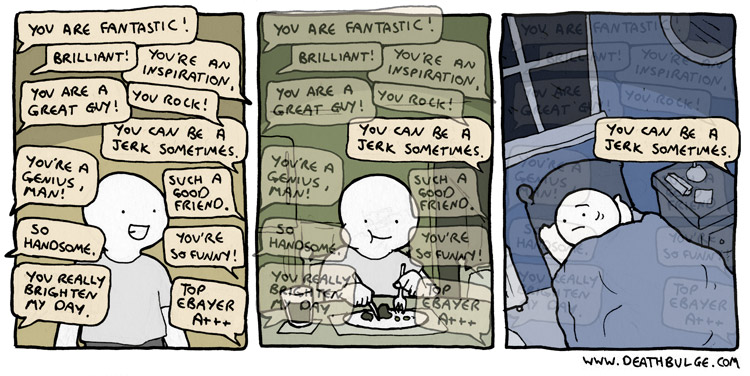
\includegraphics{fig/deathbulge-jerk.jpg}
\caption{Feedback Feelings}
\end{figure}

Feedback is most effective when the people involved can share ground
rules and expectations. This is especially important when the instructor
and/or students have different cultural or domain expectations about
feedback.

Here is a list of different ways that you, as the instructor, can set
the stage for receiving feedback in a way that helps you improve:

\begin{itemize}
\item
  Initiate feedback. It's better to ask for feedback than to receive it
  unwillingly.
\item
  Choose your own questions and ask for specific feedback. For example:

  \begin{itemize}
    \item
    ``What is one thing I could have done as an instructor to make this
    lesson more effective?''
  \item
    ``If you could pick one thing from the lesson to go over again, what
    would it be?''
  \end{itemize}
\end{itemize}

Specific feedback like this is more useful than a generic ``that was
great!'' or ``that was terrible!'' Also, writing your own feedback
questions allows you to frame feedback in a way that is helpful to you -
the questions above reveal what didn't work in your teaching, but read
as professional suggestions rather than personal judgments.

\begin{itemize}
\item
  Communicate expectations. If your teaching feedback is taking the form
  of an observation (and you're comfortable enough with the observer),
  tell that person how they can best communicate their feedback to you.
\item
  Balance positive and negative feedback.

  \begin{itemize}
    \item
    Ask for or give ``compliment sandwiches'' (one positive, one
    negative, one positive)
  \item
    Ask for both types of feedback
  \end{itemize}
\item
  Use a feedback translator. Have a fellow instructor (or other trusted
  person in the room) read over all the feedback and give an executive
  summary. It can be easier to hear ``It sounds like most people are
  following, so you could speed up'' than to read several notes all
  saying, ``this is too slow'' or ``this is boring''.
\end{itemize}

This is part of the reason for Data Carpentry and Software Carpentry's
rule, ``Never teach alone.'' Having another instructor in the classroom
saves your voice (it's hard to talk for two days straight), but more
importantly, it's a chance for instructors to learn from one another and
be a supportive voice in the room.

Finally, be kind to yourself. Mental habits matter: if you're a
self-critical person, it's OK to remind yourself that:

\begin{itemize}
\item
  It's not personal.
\item
  Look at the positives along with the negatives.
\item
  Etc.
\end{itemize}

\begin{challenge}{Feedback on Feedback}{chal:feedback-on-feedback}

Watch either \href{https://vimeo.com/139316669}{this video} or
\href{https://vimeo.com/139181120}{this one}. Take notes about
the presentation, and divide those into four groups based on whether
they are positive or negative and whether they are about the content
(what was said) or the presentation (how it was said, e.g., body
language). Compare your notes with those made by other people, and with
the feedback given by your instructor.
\end{challenge}

\begin{challenge}{Feedback on Yourself, Part II}{chal:feedback-on-yourself-part-ii}

Later in the training, repeat the first challenge exercise; however,
when it comes time to give feedback, use the same 2x2 scheme in the
previous challenge.
\end{challenge}

\begin{challenge}{Learn More About Feedback}{chal:learn-more-about-feedback}

Read Gormally et al's
``Feedback about Teaching in Higher Ed'' \cite{bib:gormally-teaching-feedback}
and discuss ways you could make peer-to-peer feedback a routine part of your teaching.
You may also enjoy Gawande's ``Personal Best'' \cite{bib:gawande-personal-best},
which looks at the value of having a coach.
\end{challenge}

\begin{challenge}{Fill In Minute Cards}{chal:fill-in-minute-cards}

We frequently use sticky notes as \emph{minute cards}: before each
break, learners take a minute to write one positive thing on the green
sticky note (e.g., one thing they've learned that they think will be
useful), and one thing they found too fast, too slow, confusing, or
irrelevant on the red one. They can use the red sticky note for
questions that haven't yet been answered. While they are enjoying their
coffee or lunch, the instructors review and cluster these to find
patterns. It only takes a few minutes to see what learners are enjoying,
what they still find confusing, what problems they're having, and what
questions are still unanswered.

Write one thing you learned this morning that you found useful on your
green sticky note, and one question you have about the material on the
red. Do \emph{not} put your name on the notes: this is meant to be
anonymous feedback. Add your notes to the pile by the door as you leave
to get coffee.
\end{challenge}

\chaplbl{Live Coding}{s:live}

One of the cornerstones of Software and Data Carpentry teaching is live
coding: instructors don't use slides, but work through the lesson
material, typing in the code or instructions, with the workshop
participants following along. This section explains how it works, why we
use it, and gives general tips for an effective live coding
presentation.

\subsection{Why Live Coding?}\label{why-live-coding}

\begin{quote}
Teaching is theater not cinema.\\--- Neal Davis
\end{quote}

We do not use slides in our lessons. Instead, instructors plug their
laptop into the projector and work through the lesson, typing in the
code, reformatting data, and talking as we go.

\begin{discussion}{Up and Down}{disc:up-and-down}

What are some of the advantages and challenges of live coding from both
a learner's and an instructor's point of view?
\end{discussion}

Its advantages are:

\begin{itemize}
\itemsep1pt\parskip0pt\parsep0pt
\item
  Watching a program being written is more compelling than watching
  someone page through slides that present bits and pieces of the same
  code.
\item
  It enables instructors to be more responsive to ``what if?''
  questions. Where a slide deck is like a railway track, live coding
  allows instructors to go off road and follow their learners'
  interests.
\item
  It facilitates lateral knowledge transfer: people learn more than we
  realized we were teaching by watching \emph{how} instructors do
  things.
\item
  It slows the instructor down: if she has to type in the program as she
  goes along, she can only go twice as fast as her learners, rather than
  ten-fold faster as she could with slides.
\item
  Learners get to see instructors' mistakes \emph{and how to diagnose
  and correct them}. Novices are going to spend most of their time doing
  this, but it's left out of most textbooks.
\end{itemize}

It takes a bit of practice for instructors to get used to thinking aloud
while coding in front of an audience, but most report that it is then no
more difficult to do than talking off a deck of slides.

Many instructors now use two devices when teaching: a laptop plugged
into the projector for learners to see, and a tablet beside it on which
they can view their notes and the Etherpad session. This seems to be
more reliable than displaying one virtual desktop while flipping back
and forth to another.

\begin{challenge}{I/We/You vs.~You/Y'all/We}{chal:iweyou-vs-youyallwe}

Live coding is an example of the ``I/We/You'' approach to teaching
\href{\{\{\%20page.root\%20\}\}/05-performance/}{discussed earlier}.
\end{challenge}

\begin{challenge}{Up and Down}{chal:up-and-down}

What are some of the advantages and challenges of live coding from both
a learner's and an instructor's point of view?
\end{challenge}

\begin{challenge}{The Bad and the Good}{chal:the-bad-and-the-good}

Watch this video of \href{https://youtu.be/bXxBeNkKmJE}{live coding done
poorly} and this video of \href{https://youtu.be/SkPmwe\_WjeY}{live
coding done right} as a group and then summarize your feedback on both.
In the videos, the bash shell \texttt{for} loop is taught, and it is
assumed learners are familiar with how to use a variable, the
\texttt{head}command and the content of the
\texttt{basilisk.dat unicorn.dat} files.
\end{challenge}

\subsection{Live Coding Top 10}\label{live-coding-top-10}

Below follow ten tips to help you get started with effective live
coding:

\subsubsection{Be Seen and Heard}\label{be-seen-and-heard}

If you are physically able to stand up for a couple of hours, do it
while you are teaching. When you sit down, you are hiding yourself
behind others for those sitting in the back rows. Make sure to notify
the workshop organizers of your wish to stand up and ask them to arrange
a high table/standing desk or
\href{https://en.wikipedia.org/wiki/Lectern\#Academic\_context}{lectern}.

Regardless of whether you are standing or sitting, make sure to move
around as much as reasonable. You can for example go to the screen to
point something out, or draw something on the white/blackboard (see
below). Moving around makes the teaching more lively, less monotonous.
It draws the learners' attention away from their screens, to you, which
helps get the point you are making across.

Even though you may have a good voice and know how to use it well, it
may be a good idea to use a microphone, especially if the workshop room
is equipped with one. Your voice will be less tired, and you increase
the chance of people with hearing difficulties being able to follow the
workshop.

\subsubsection{Take It Slow}\label{take-it-slow}

For every command you type, every word of code you write, every menu
item or website button you click, say out loud what you are doing while
you do it. Then point to the command and its output on the screen and go
through it a second time. This not only slows you down, it allows
learners who are following along to copy what you do, or to catch up,
even when they are looking at their screen while doing it. If the output
of your command or code makes what you just typed disappear from view,
scroll back up so learners can see it again - this is especially needed
for the Unix shell lesson.

Other possibilities are to execute the same command a second time, or
copy and paste the last command(s) into the workshop Etherpad.

\subsubsection{Mirror Your Learner's Environment As Much As
Possible}\label{mirror-your-learners-environment-as-much-as-possible}

You may have set up your environment to your liking, with a very simple
or rather fancy Unix prompt, colour schemes for your development
environment, keyboard shortcuts etc. Your learners usually won't have
all of this. Try to create an environment that mirrors what your
learners have, and avoid using keyboard shortcuts. Some instructors
create a separate `bare-bone' user (login) account on their laptop, or a
separate `teaching-only' account on the service being taught
(e.g.~Github).

\subsubsection{Use The Screen Wisely}\label{use-the-screen-wisely}

Use a big font, and maximize the window. A black font on a white
background works better than a light font on a dark background. When the
bottom of the projector screen is at the same height, or below, the
heads of the learners, people in the back won't be able to see the lower
parts. Draw up the bottom of your window(s) to compensate.

If you can get a second screen, use it! It will usually require its own
PC or laptop, so you may need to ask a helper to control it. You could
use the second screen to show the Etherpad content, or the lesson
material, or illustrations.

Pay attention to the lighting (not too dark, no lights directly on/above
the presenter's screen) and if needed, reposition the tables so all
learners can see the screen, and helpers can easily reach all learners.

\subsubsection{Use Illustrations}\label{use-illustrations}

Most lesson material comes with illustrations, and these may help
learners to understand the stages of the lesson and to organize the
material. What can work really well is when you as instructor generate
the illustrations on the white/blackboard as you progress through the
material. This allows you to build up diagrams, making them increasingly
complex in parallel with the material you are teaching. It helps
learners understand the material, makes for a more lively workshop
(you'll have to move between your laptop and the blackboard) and gathers
the learners' attention to you as well.

\subsubsection{Avoid Being Disturbed}\label{avoid-being-disturbed}

Turn off any notifications you may use on your laptop, such as those
from social media, email, etc. Seeing notifications flash by on the
screen distracts you as well as the learners - and may even result in
awkward situations when a message pops up you'd rather not have others
see.

\subsubsection{Stick to the Lesson
Material}\label{stick-to-the-lesson-material}

The core Software and Data Carpentry lessons are developed
collaboratively by many instructors and tried and tested at many
workshops. This means they are very streamlined - which is great when
you start teaching them for the first time. It may be tempting to
deviate from the material because you would like to show a neat trick,
or demonstrate some alternative way of doing something. Don't do this,
since there is a fair chance you'll run into something unexpected that
you then have to explain. If you really want to use something outside of
the material, try it out thoroughly before the workshop: run through the
lesson as you would during the actual teaching and test the effect of
your modification.

Some instructors use printouts of the lesson material during teaching.
Others use a second device (tablet or laptop) when teaching, on which
they can view their notes and the Etherpad session. This seems to be
more reliable than displaying one virtual desktop while flipping back
and forth to another.

\subsubsection{Leave No Learner Behind}\label{leave-no-learner-behind}

Give each learner two sticky notes of different colours, e.g., red and
green. These can be held up for voting, but their real use is as status
flags. If someone has completed an exercise and wants it checked, they
put the green sticky note on their laptop; if they run into a problem
and need help, the put up the red one. This is better than having people
raise their hands because:

\begin{itemize}
\itemsep1pt\parskip0pt\parsep0pt
\item
  it's more discreet (which means they're more likely to actually do
  it),
\item
  they can keep working while their flag is raised, and
\item
  the instructor can quickly see from the front of the room what state
  the class is in.
\end{itemize}

Sometimes a red sticky involves a technical problem that takes a bit
more time to solve. To prevent this issue to slow down the whole class
too much, you could use the occasion to take the small break you had
planned to take a bit later, giving the helper(s) time to fix the
problem.

\subsubsection{Embrace Mistakes}\label{embrace-mistakes}

No matter how well prepared you are, you will be making mistakes. Typo's
are hard to avoid, you may overlook something from the lesson
instructions, etc. This is OK! It allows learners to see instructors'
mistakes and how to diagnose and correct them. Some mistakes are
actually an opportunity to point something out, or reflect back on
something covered earlier. Novices are going to spend most of their time
making the same and other mistakes, but how to deal with them is left
out of most textbooks.

\begin{quote}
The typos are the pedagogy\\--- Emily Jane McTavish
\end{quote}

\subsubsection{Have Fun}\label{have-fun}

Teaching is performance art and can be rather serious business. On the
one hand, don't let this scare you - it is much easier than performing
Hamlet. You have an excellent script at your disposal, after all! On the
other hand, it is OK to add an element of `play', i.e. use humor and
improvisation to liven up the workshop. How much you are able and
willing to do this is really a matter of personality and taste - as well
as experience. It becomes easier when you are more familiar with the
material, allowing you to relax more. Choose your words and actions
wisely, though. Remember that we want the learners to have a welcoming
experience and a positive learning environment - a misplaced joke can
ruin this in an instant. Start small, even just saying `that was fun'
after something worked well is a good start. Ask your co-instructors and
helpers for feedback when you are unsure of the effect you behaviour has
on the workshop.

\begin{challenge}{See Then Do}{chal:see-then-do}

Teach 3-4 minutes of your chosen lesson episode using live coding to a
fellow trainee, then swap and watch while that person live codes for
you. Don't bother trying to record the live coding sessions---we have
found that it's difficult to capture both the person and the screen with
a handheld device---but give feedback the same way you have previously
(positive and negative, content and presentation). If you decide to
instead teach something from the lesson episode you selected in
preparation for this workshop, explain in advance to your fellow trainee
what you will be teaching and what the learners you teach it to are
expected to be familiar with.
\end{challenge}

\begin{quote}
How does live coding compare to other kinds of demonstration-based
teaching like lab lessons?
\end{quote}

\chaplbl{Teaching Practices}{sec:practices}

We regard teaching as a performance art, no different from drama, music,
or athletics. And as in those fields, we have a collection of small tips
and tricks to make teaching work better.

\seclbl{Challenges}{sec:challenges}

With live coding, it is easy for some learners to fall behind, and for
other learners to get bored. Given the diversity of our learners'
backgrounds and skills, we will always have a mix of more and less
advanced people in our classes. No matter what we teach, and how fast or
how slow we go, 20\% or more of the room will be lost, and there's a
good chance that a different 20\% will be bored.

The obvious solution is to split people by level, but if we ask them how
much they know about particular things, they regularly under- or
over-estimate their knowledge. We have therefore developed a short
pre-assessment questionnaire that asks them how easily they could do a
small number of specific tasks. It gives instructors some idea of who
they're going to be helping, but we have not validated the questions,
i.e., we have not done the laborious work of interviewing respondents to
ensure that they are interpreting the questions the same way that we
are. We also have not yet done the follow-up to see whether the
questionnaires' categorization of learners matches their actual in-class
proficiency.

\begin{callout}{You Can't Just Ask}{callout:you-cant-just-ask}

Instead of asking people how easily they could complete specific tasks,
we could just ask them to rate their knowledge of various subjects on a
scale from 1 to 5. However, self-assessments of this kind are usually
inaccurate because of the
\href{https://en.wikipedia.org/wiki/Dunning\%E2\%80\%93Kruger\_effect}{Dunning-Kruger
effect}: the less people know about a subject, the less accurate their
estimate of their knowledge is.
\end{callout}

That said, there \emph{are} things we can do:

\begin{itemize}
\item
  Before running a workshop, communicate its level clearly to everyone
  who's thinking of signing up by listing the topics that will be
  covered and showing a few examples of exercises that people will be
  asked to complete.
\item
  Provide multiple exercises for each teaching episode so that more
  advanced learners don't finish early and get bored.
\item
  Ask more advanced learners to help people next to them. They'll learn
  from answering their peers' questions (since it will force them to
  think about things in new ways).
\item
  The helpers and the instructor who isn't teaching the particular
  episode should keep an eye out for learners who are falling behind and
  intervene early so that they don't become frustrated and give up.
\end{itemize}

The most important thing is to accept that no class can possibly meet
everyone's individual needs. If the instructor slows down to accommodate
two people who are struggling, the other 38 are not being well served.
Equally, if she spends a few minutes talking about an advanced topic
because two learners are bored, the 38 who don't understand it will feel
left out. All we can do is tell our learners what we're doing and why,
and hope that they'll understand.

\seclbl{Other Practices}{sec:other-practices}

\begin{description}
\item[Sticky notes.]
We give each learner two sticky notes of different colors, e.g., red and
green. These can be held up for voting, but their real use is as status
flags. If someone has completed an exercise and wants it checked, they
put the green sticky note on their laptop; if they run into a problem
and need help, the put up the red one. This is better than having people
raise their hands because:

\begin{itemize}
\item
  it's more discreet (which means they're more likely to actually do
  it),
\item
  they can keep working while their flag is raised, and
\item
  the instructor can quickly see from the front of the room what state
  the class is in.
\end{itemize}
\item[Minute cards.]
As explained in \secref{sec:performance},
we also use sticky notes as minute cards: before each coffee or meal
break, learners take a minute to write one positive thing on the green
sticky note (e.g., one thing they've learned that they think will be
useful), and one thing they found too fast, too slow, confusing, or
irrelevant on the red one. They can use the red sticky note for
questions that haven't yet been answered. It only takes a few minutes to
cluster these, and allows the instructors to adjust to learners'
interests and speed.
\item[One up, one down.]
We frequently also ask for summary feedback at the end of each day. The
instructors ask the learners to alternately give one positive and one
negative point about the day, without repeating anything that has
already been said. This requirement forces people to say things they
otherwise might not: once all the ``safe'' feedback has been given,
participants will start saying what they really think.

Minute cards are anonymous; the alternating up-and-down feedback is not.
Each mode has its strengths and weaknesses, and by providing both, we
hope to get the best of both worlds.
\item[Learners use their own machines.]
Learners tell us that it is important to them to leave the workshop with
their own machine set up to do real work. We therefore continue to teach
on all three major platforms (Linux, Mac OS X, and Windows), even though
it would be simpler to require learners to use just one.

We have experimented with virtual machines (VMs) on learners' computers
to reduce installation problems, but those introduce problems of their
own: older or smaller machines simply aren't fast enough, and learners
often struggle to switch back and forth between two different sets of
keyboard shortcuts for things like copying and pasting.

Some instructors use VPS over SSH or web browser pages instead. This
solve the installation issues, but makes us dependent on host
institutions' WiFi (which can be of highly variable quality), and has
the issues mentioned above with things like keyboard shortcuts.

\item[Collaborative note-taking.]
\fixme{back ref to welcome - mention that boredom spreads}

\item[Pair programming.]
Pairing is a good practice in real life, and also a
good way to teach \cite{bib:porter-what-works}. Partners can not only help each other out during the
practical, but can also clarify each other's misconceptions when the
solution is presented, and discuss common research interests during
breaks. To facilitate this, we strongly prefer flat (dinner-style)
seating to banked (theater-style) seating; this also makes it easier for
helpers to reach learners who need assistance.

When pair programming is used it's important to put \emph{everyone} in
pairs, not just the learners who are struggling, so that no one feels
singled out. It's also useful to have people sit in new places (and
hence pair with different partners) after each coffee or meal break.
\item[Peak rule.]
The \href{https://en.wikipedia.org/wiki/Peak\%E2\%80\%93end\_rule}{peak
rule} states that people judge an experience primarily based on how they
felt at its most intense point and how they felt at its end. While it
has been criticized for not strongly predicting what's remembered, it's
always worth trying to end a lesson on a high note.
\item[Instructor notes.]
Many of the Software and Data Carpentry lessons have instructor's notes,
with information from instructors who have already taught the material.
This can be a valuable resource when preparing lessons, especially when
teaching a lesson for the first time.\\The Software Carpentry instructor
guides are linked on each lesson page; the instructor guides for Data
Carpentry lessons are on their
main lesson page.
\end{description}

\begin{callout}{Why Not a MOOC?}{callout:why-not-a-mooc}

Many learners find it difficult to get to a workshop, either because
there isn't one locally or because it's difficult to schedule time
around other commitments, so why don't we create video recordings of the
lessons and offer the workshop as a MOOC (Massive Open Online Course)?

The first answer is that we did in 2010-11, but found the maintenance
costs unsustainable. Making a small change to this webpage only takes a
few minutes. but making \emph{any} change to a video takes an hour or
more. In addition, most people are much less comfortable recording
themselves than contributing written material.

The second answer is that doing significantly outperforms watching.
Specifically, a
recent paper by Koedinger et al \cite{bib:koedinger-doing-watching}
estimated ``\ldots{}the learning benefit from
extra doing (1 SD increase) to be more than six times that of extra
watching or reading.'' \emph{Doing}, in this case, refers to completing
an interactive or mimetic task with feedback, while \emph{benefit}
refers to both \emph{completion rates} and \emph{overall performance}.

And while we do not (yet) have empirical data, we believe very strongly
that many novices would give up in despair if required to debug setup
and installation lessons on their own, but are more likely to get past
these obstacles if someone is present to help them.

An intermediate approach that we are experimenting with is real-time
remote instruction, in which the learners are co-located at one (or a
few) sites, with helpers present, while the instructor(s) teaching via
online video. This model has worked well for this instructor training
course, and for a handful of regular workshops, but more work is needed
to figure out its pros and cons.
\end{callout}

\chaplbl{Motivation and Demotivation}{s:motivation}

In order for learners to step out into new and familiar terrain, they
will need encouragement. This section discusses typical ways that
learners are motivated (and can be demotivated!) and describes ways that
communities of practice can be welcoming (or threatening) to new
members.

\subsection{Motivation}\label{motivation}

People learn best when they care about the topic and believe they can
master it. This presents us with a problem because most scientists don't
want to program: they want to do science, and rightly regarding
programming as a tax they have to pay in order to do so. In addition,
their early experiences with programming are often demoralizing, and
believing that something will be hard to learn is a self-fulfilling
prophecy.

Imagine a grid whose axes are labelled ``mean time to master'' and
``usefulness once mastered''. Everything that's quick to master, and
immediately useful should be taught first; things in the opposite corner
that are hard to learn and have little near-term application don't
belong in this course.

\begin{figure}[htbp]
\centering
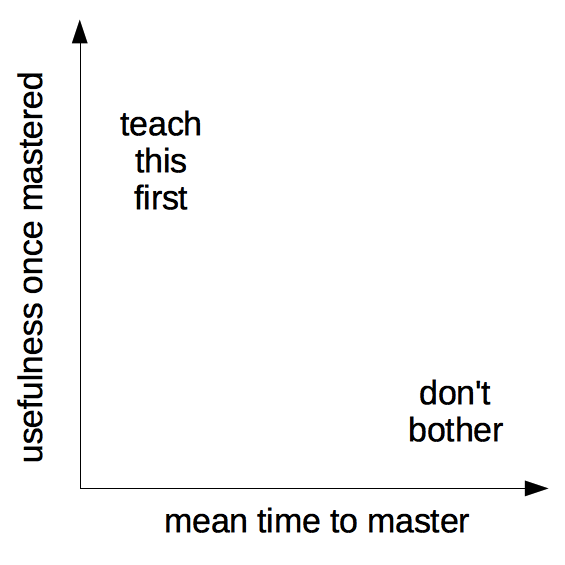
\includegraphics{../fig/what-to-teach.png}
\caption{What to Teach}
\end{figure}

\begin{quote}
\subsection{Actual Time}\label{actual-time}

Any useful estimate of how long something takes to master must take into
account how frequent failures are and how much time is lost to them. For
example, editing a text file seems like a simple task, but most
graphical editors save things to the user's desktop or home directory.
If people need to run shell commands on the files they've edited, a
substantial fraction won't be able to navigate to the right directory
without help. If this seems like a small problem to you, please revisit
the discussion of expert blind spot \secref{sec:memory}. \{: .callout\}
\end{quote}

Many of the foundational concepts of computer science, such as
computability, inhabit the ``useful but hard to learn'' corner of the
grid described above. This doesn't mean that they aren't worth learning,
but if our aim is to convince people that they \emph{can} learn this
stuff, and that doing so will help them do more science faster, they are
less compelling than things like automating repetitive tasks.

We have therefore adopted a ``teach most immediately useful first''
approach. We try to have learners do something that \emph{they} think is
useful in their daily work within 15 minutes of starting each lesson.
This not only motivates them, it also helps build their confidence in
us, so that if it takes longer to get to the payoff of a later topic,
they'll stick with us.

Perhaps the best-studied use of this idea is the
media computation approach developed by Guzdial and Ericson at Georgia Tech
\cite{bib:guzdial-mediacomp-retrospective}.
Instead of printing ``hello world'' or summing the first ten integers,
their students' first program opens an image, resizes it to create at
thumbnail, and saves the result. This is an \emph{authentic task}, i.e.,
something that learners believe they would actually do in real life. It
is also \emph{tangible}: if the image comes out the wrong size, learners
have a concrete starting point for debugging.

\begin{challenge}{Authentic Tasks: Think, Pair, Share}{chal:authentic-tasks-think-pair-share}

\textbf{Think} about something you did this week that uses one or more
of the skills we teach, (e.g.~wrote a function, bulk downloaded data,
did some stats in R, forked a repo) and explain how you would use it (or
a simplified version of it) as an exercise or example in class.
\textbf{Pair} up with your neighbor and decide where this exercise fits
on a 2x2 grid of ``short/longtime to master'' and ``low/high
usefulness''? In the class Etherpad, \textbf{share} the task and where
it fits on the 2x2 grid. As a group, we will discuss how these relate
back to our ``teach most immediately useful first'' approach.
\end{challenge}

\subsection{Strategies for Motivating
Learners}\label{strategies-for-motivating-learners}

\emph{\href{http://www.amazon.com/How-Learning-Works-Research-Based-Jossey-Bass/dp/0470484101/}{How
Learning Works}} contains this list of evidence-based methods to
motivate learners. None of them are surprising---it's hard to imagine
someone saying that we \emph{shouldn't} identify and reward what we
value---but it's useful to check lessons against these points to make
sure they're doing at least a few of these things.

\begin{quote}
\subsection{Provide an Example}\label{provide-an-example}

Insert a personal story here about how you establish value in the
classroom. Or, use Rayna's personal story, which goes like this: In the
Unix lesson, we use a haiku to teach grep. This is a great didactic
tool, but it can be hard for learners to see how they can use it in
their research. After the grep lesson, I show a one liner that combines
\texttt{head}, \texttt{grep}, \texttt{sort}, and \texttt{uniq} to
produce a ranked list of the most abundant sequences. I emphasize that
the students just learned each of the pieces (see
\href{https://wikis.utexas.edu/display/bioiteam/Scott's list of linux one-liners}).
This way, I connect my bioinformatics users with domain-specific
examples using an authentic task that is relevant to their research. \{:
.callout\}
\end{quote}

\begin{challenge}{Brainstorming Motivational Strategies}{chal:brainstorming-motivational-strategies}

\emph{Think} back to a computational (or other) course you took in the
past, and identify one thing the instructor did that motivated you.
\emph{Pair} up with your neighbor and discuss what motivated you.
\emph{Share} the motivational story in the Etherpad.
\end{challenge}

\begin{quote}
\subsection{Not Just Learners}\label{not-just-learners}

What's missing from this list is strategies to motivate the
\emph{instructor}. As we said in \secref{sec:intro},
learners respond to an instructor's enthusiasm, and instructors need to
care about a topic in order to keep teaching it, particularly when they
are volunteers. \{: .callout\}
\end{quote}

\begin{challenge}{Why Do You Teach?}{chal:why-do-you-teach}

We all have a different motivation for teaching, and that is a really
good thing! SWC wants instructors with diverse backgrounds because you
each bring something unique to our community. After this
class, or during a break, write a short explanation of what motivates
you to teach. Save this as part of your teaching philosophy for future
reference.
\end{challenge}

\subsection{Demotivation}\label{demotivation}

As noted in \secref{sec:intro}, we are privileged: most of our learners are physically
safe, well fed, well educated, and highly motivated. Our challenge is
therefore not demotivating them.

A few common demotivators are \emph{indifference} and \emph{unfairness}.
If learners believe that the instructor or the educational system
doesn't care about them or the lesson, they won't care either. And if
people believe the class is unfair, they will also be demotivated, even
if it is unfair in their favor (because consciously or unconsciously
they will worry that they will some day find themselves in the group on
the losing end). Finally, a ``holier-than-thou'' or contemptuous
attitude from an instructor is a quick way to alienate a classroom and
cause learners to tune out.

\begin{quote}
\subsection{Things You Shouldn't Do in a
Workshop}\label{things-you-shouldnt-do-in-a-workshop}

\begin{itemize}
\itemsep1pt\parskip0pt\parsep0pt
\item
  Tell learners they are rubbish because they use Excel and/or Word,
  don't modularize their code, etc.
\item
  Repeatedly make digs about Windows and praise Linux, e.g., say that
  the former is for amateurs.
\item
  Criticize GUI applications (and by implication their users) and
  describe command-line tools as the One True Way.
\item
  Dive into complex or detailed technical discussion with the one or two
  people in the audience who clearly don't actually need to be there.
\item
  Pretend to know more than you do. People will actually trust you more
  if you are frank about the limitations of your knowledge, and will be
  more likely to ask questions and seek help.
\item
  Use the J word (``just''). As discussed in \secref{sec:memory}, this
  signals to the learner that the instructor thinks their problem is
  trivial and by extension that they therefore must be stupid for not
  being able to figure it out.
\item
  Feign surprise. Saying things like ``I can't believe you don't know
  X'' or ``you've never heard of Y?'' signals to the learner that they
  do not have some required pre-knowledge of the material you are
  teaching, that they are in the wrong place, and it may prevent them
  from asking questions in the future. (This idea is due to the Recurse
  Center's \href{https://www.recurse.com/manual\#sec-environment}{Social
  Rules}). \{: .callout\}
\end{itemize}
\end{quote}

\begin{quote}
\subsection{The Importance of Having
Rules}\label{the-importance-of-having-rules}

Software Carpentry and Data Carpentry share a
Code of Conduct, and all
participants in our workshops are required to abide by it. Its details
are important, but the most important thing about it is that it exists:
knowing that we have rules tells people a great deal about our values
and about what kind of learning experience they can expect. \{:
.callout\}
\end{quote}

\begin{quote}
\subsection{Stereotype Threat}\label{stereotype-threat}

Reminding people of negative stereotypes, even in subtle ways, makes
them anxious about the risk of confirming those stereotypes, which in
turn reduces their performance. This is called
\emph{\href{https://en.wikipedia.org/wiki/Stereotype\_threat}{stereotype
threat}}, and the clearest examples in computing are gender-related.
Depending on whose numbers you trust, only 12-18\% of programmers are
women, and those figures have actually been getting worse over the last
20 years. There are many reasons for this (see Margolis and Fisher's
\emph{\href{http://www.amazon.com/Unlocking-Clubhouse-Computing-Jane-Margolis/dp/0262632691/}{Unlocking
the Clubhouse}} and Margolis's
\emph{\href{https://www.amazon.com/Stuck-Shallow-End-Education-Computing/dp/0262514044/}{Stuck
in the Shallow End}}), and Steele's
\emph{\href{http://www.amazon.com/dp/0393339726/}{Whistling Vivaldi}}
summarizes what we know about stereotype threat in general and presents
some strategies for mitigating it in the classroom.

However, while there's lots of evidence that unwelcoming climates
demotivate members of under-represented groups, it's not clear that
stereotype threat is the underlying mechanism. Part of the problem is
that
\href{http://www.europhd.net/html/\_onda02/07/PDF/20th\_lab\_materials/jane/shapiro\_neuberg\_2007.pdf}{the
term has been used in many ways}; another is
\href{https://www.psychologytoday.com/blog/rabble-rouser/201512/is-stereotype-threat-overcooked-overstated-and-oversold}{questions
about the replicability of key studies}. What \emph{is} clear is that we
need to aovid thinking in terms of a deficit model (i.e., we need to
change the members of under-represented groups because they have some
deficit, such as lack of prior experience) and instead use a systems
approach (i.e., we need to change the system because it produces these
disparities). \{: .callout\}
\end{quote}

\begin{challenge}{Brainstorming Demotivational Experiences}{chal:brainstorming-demotivational-experiences}

\emph{Think} back to a time when you demotivated a student (or when you
were demotivated as a student). \emph{Pair} up with your neighbor and
discuss what you could have done differently in the situation.
\emph{Share} the demotivational story in the Etherpad.
\end{challenge}

\begin{quote}
\subsection{Never Learn Alone}\label{never-learn-alone}

One way to support at-risk learners of all kinds is to have people sign
up for workshops in small teams rather than as individuals. If an entire
lab group comes, or if attendees are drawn from the same (or
closely-related) disciplines, everyone in the room will know in advance
that they will be with at least a few people they trust, which increases
the chances of them actually coming. It also helps after the workshop:
if people come with their labmates, they can work together to implement
what they've learned. \{: .callout\}
\end{quote}

\subsubsection{Impostor Syndrome}\label{impostor-syndrome}

\href{https://en.wikipedia.org/wiki/Impostor\_syndrome}{Impostor
syndrome} is the belief that one is not good enough for a job or
position, that one's achievements are lucky flukes, and an accompanying
fear of being ``found out''. Impostor syndrome seems to be particularly
common among
\href{https://www.usenix.org/blog/impostor-syndrome-proof-yourself-and-your-community}{high
achievers who undertake publicly visible work}.

Academic work is frequently undertaken alone or in small groups but the
results are shared and criticized publicly. In addition, we rarely see
the struggles of others, only their finished work, which can feed the
belief that everyone else finds it easy. Women and minority groups, who
already feel additional pressure to prove themselves in some settings,
\href{http://www.paulineroseclance.com/pdf/ip\_high\_achieving\_women.pdf}{may
be particularly affected}.

Two ways of dealing with your own impostor syndrome are:

\begin{enumerate}
\def\labelenumi{\arabic{enumi}.}
\itemsep1pt\parskip0pt\parsep0pt
\item
  Ask for feedback from someone you respect and trust. Ask them for
  their honest thoughts on your strengths and achievements, and commit
  to believing them.
\item
  Look for role models. Who do you know who presents as confident and
  capable? Think about how they conduct themselves. What lessons can you
  learn from them? What habits can you borrow? (Remember, they quite
  possibly also feel as if they are making it up as they go.)
\end{enumerate}

As an instructor, you can help people with their impostor syndrome by
sharing stories of mistakes that you have made or things you struggled
to learn. This reassures the class that it's OK to find topics hard.
Being open with the group makes it easier to build trust and make
students confident to ask questions. (Live coding is great for this:
typos let the class see you're not superhuman.)

You can also emphasize that you want questions: you are not succeeding
as a teacher if no one can follow your class, so you're asking students
for their help to help you learn and improve. Remember, it's much more
important to \emph{be} smart than to \emph{look} smart.

The Ada Initiative has
\href{http://adainitiative.org/continue-our-work/impostor-syndrome-training/}{some
excellent resources} for teaching about and dealing with imposter
syndrome.

\subsubsection{Mindset}\label{mindset}

Learners can be demotivated in subtler ways as well. For example, Dweck
and others have studied the differences of
\href{https://en.wikipedia.org/wiki/Mindset\#Fixed\_mindset\_and\_growth\_mindset}{fixed
mindset and growth mindset}. If people believe that competence in some
area is intrinsic (i.e., that you either ``have the gene'' for it or you
don't), \emph{everyone} does worse, including the supposedly advantaged.
The reason is that if they don't get it at first, they figure they just
don't have that aptitude, which biases future performance. On the other
hand, if people believe that a skill is learned and can be improved,
they do better on average.

A person's mindset can be shaped by subtle cues. For example, if a child
is told, ``You did a good job, you must be very smart,'' she is likely
to develop a fixed mindset. If on the other hand she is told, ``You did
a good job, you must have worked very hard,'' she is likely to develop a
growth mindset, and subsequently achieve more. Studies have also shown
that the simple action of telling learners about the different mindsets
before a course can improve learning outcomes for the whole group.

\subsection{Accessibility}\label{accessibility}

Not providing equal access to lessons and exercises is about as
demotivating as it gets. If you look at
\href{http://swcarpentry.github.io/v4/python/flow.html}{our old lesson
on Python}, for example, you'll find that the text beside the slides
includes all of the narration---but none of the Python source code.
Someone using a
\href{https://en.wikipedia.org/wiki/Screen\_reader}{screen reader} would
therefore be able to hear what was being said about the program, but
wouldn't know what the program actually was.

While it may not be possible to accommodate everyone's needs, it
\emph{is} possible to get a good working structure in place without any
specific knowledge of what specific disabilities people might have.
Having at least some accommodations prepared in advance also makes it
clear that hosts and instructors care enough to have thought about
problems in advance, and that any additional concerns are likely to be
addressed.

\begin{quote}
\subsection{It Helps Everyone}\label{it-helps-everyone}

\href{https://en.wikipedia.org/wiki/Curb\_cut}{Curb cuts} (the small
sloped ramps joining a sidewalk to the street) were originally created
to make it easier for the physically disabled to move around, but proved
to be equally helpful to people with strollers and grocery carts.
Similarly, steps taken to make lessons more accessible to people with
various disabilities also help everyone else. Proper captioning of
images, for example, doesn't just give screen readers something to say:
it also makes the images more findable by exposing their content to
search engines. \{: .callout\}
\end{quote}

The first step is to know what you need to do. The
\href{http://www.w3.org/WAI/training/accessible}{W3C Accessibility
Initiative's checklist for presentations} is a good starting point
focused primarily on assisting the visually impaired, while Liz Henry's
blog post about
\href{https://modelviewculture.com/pieces/unlocking-the-invisible-elevator-accessibility-at-tech-conferences}{accessibility
at conferences} has a good checklist for people with mobility issues,
and
\href{https://modelviewculture.com/pieces/qa-making-tech-events-accessible-to-the-deaf-community}{this
interview} with Chad Taylor is a good introduction to issues faced by
the hearing impaired.

The second is to know how well you're doing. For example, sites like
\href{http://webaim.org/}{WebAIM} allow you to check how accessible your
online materials are to visually impaired users. (According to
\href{http://wave.webaim.org/report\#/software-carpentry.org}{this
report}, we still have some work to do\ldots{})

The third, and most important, is to \emph{involve people with
disabilities in decision-making}. Our mailing lists are a good place to
ask for advice, and updates to
\href{http://software-carpentry.org/workshops/checklists/accessibility/}{our
accessibility checklist} are always welcome.

\begin{quote}
\subsection{Every Little Bit Counts}\label{every-little-bit-counts}

Looking at people who work with disability and accessibility, it's easy
to be overwhelmed by all the different ways we could make instruction
more accessible. \emph{Don't panic.} Instead:

\begin{itemize}
\itemsep1pt\parskip0pt\parsep0pt
\item
  \emph{Don't do everything at once.} We don't ask learners in our
  workshops to adopt all our best practices or tools in one go, but
  instead to work things in gradually at whatever rate they can manage.
  Similarly, try to build in accessibility habits when preparing for
  workshops by adding something new each time.
\item
  \emph{Do the easy things first.} There are plenty of ways to make
  workshops more accessible that are both easy and don't create extra
  cognitive load for anyone: font choices, general text size, checking
  in advance that your room is accessible via an elevator or ramp, etc.
  \{: .callout\}
\end{itemize}
\end{quote}

\begin{quote}
\subsection{Accessibility Testing}\label{accessibility-testing}

Find the nearest public transportation drop-off point to your building
and walk from there to your office and then to the nearest washroom,
making notes about things you think would be difficult for someone with
mobility issues. Now borrow a wheelchair and repeat the journey. How
complete was your list of challenges? And did you notice that the first
sentence in this challenge assumed you could actually walk? \{:
.callout\}
\end{quote}

\subsection{Inclusivity}\label{inclusivity}

\emph{Inclusivity} is a policy of including people who might otherwise
be excluded or marginalized. In computing, it means making a positive
effort to be more welcoming to women, people of color, people with
various sexual orientations, the elderly, the physically challenged, the
formerly incarcerated, the economically disadvantaged, and everyone else
who doesn't fit Silicon Valley's white/Asian male demographic. Lee's
paper
``What can I do today to create a more inclusive community in CS?''
\cite{bib:lee-create-inclusive-community}
is a brief, practical guide to
doing that with references to the research literature. These help
learners who belong to one or more margainalized or excluded groups, but
help motivate everyone else as well; while they are phrased in terms of
term-long courses, many can be applied in our workshops, such as:

\begin{itemize}
\itemsep1pt\parskip0pt\parsep0pt
\item
  asking learners to email you before the workshop to explain how they
  believe the training could help them achieve their goals;
\item
  reviewing notes to make sure they are free from gendered pronouns,
  that they include culturally diverse names, etc.;
\item
  emphasize that what matters is the rate at which they are learning,
  not the advantages or disadvantages they had when they started;
\item
  encouraging pair programming; and
\item
  actively mitigate behavior that some learners may find intimidating,
  e.g., use of jargon or ``questions'' that are actually asked to
  display knowledge.
\end{itemize}

\begin{challenge}{Pick One}{chal:pick-one}

\begin{enumerate}
\def\labelenumi{\arabic{enumi}.}
\itemsep1pt\parskip0pt\parsep0pt
\item
  Pick one activity or change in practice from
  Lee's paper \cite{bib:lee-create-inclusive-community}
  that you would like to work on.
\item
  Put a reminder in your calendar three months in the future to
  self-check whether you have done something about it.
\end{enumerate}
\end{challenge}


\part{Community}

\chaplbl{The Carpentries}{s:carpentries}

In becoming an instructor for Software or Data Carpentry, you are also
becoming part of a community of like-minded volunteers. This section
provides some background on both organizations, and on the final steps
toward certification.

\begin{callout}{Preparation and Discussion}{callout:preparation-and-discussion}

This discussion assumes that trainees have read the operations
guide (which is assigned as overnight homework). Instead of going through this material point by
point, trainers should ask each trainee to add one non-overlapping
question to a list, then go through that list.
\end{callout}

\subsection{History}\label{history}

\href{http://software-carpentry.org}{Software Carpentry} was co-founded
in 1998 by Brent Gorda and Greg Wilson, who identified a need for best
practices training in research computing. After several iterations, the
current model of two-day workshops with a standard curriculum emerged in
2010-11. After intermediate support from various organizations, it
became an independent non-profit organization called the
\href{http://software-carpentry.org/scf/}{Software Carpentry Foundation}
(SCF) in 2015. The SCF is now responsible for all aspects of Software
Carpentry's operations.

\begin{callout}{History Lesson}{callout:history-lesson}

For more on Software Carpentry's history, and on what we've learned
along the way, see
\href{http://software-carpentry.org/scf/history/}{this page} on its
website or the paper
``\href{http://f1000research.com/articles/3-62/v2}{Software Carpentry: Lessons Learned}''.
\end{callout}

In 2013, members of the Software Carpentry community identified a need
for training aimed at computational novices that would teach researchers
how to properly handle their data. This led to the creation of
\href{http://datacarpentry.org}{Data Carpentry} under the leadership
of Tracy Teal. While separate, the two organization share many aspects
of their operations, long-term goals, and community structure:

\begin{itemize}
\item
  Both focus on computational skills.
\item
  Both run two-day workshops taught by volunteer instructors.
\item
  Both strive to fill gaps in current training for researchers.
\end{itemize}

However, they differ in their content and intended audience. Data
Carpentry workshops focus on best practices surrounding data. Its
learners are not people who want to learn about coding, but rather those
who have a lot of data and don't know what to do with it. Accordingly,
Data Carpentry workshops:

\begin{itemize}
\item
  are aimed at pure novices,
\item
  domain-specific, and
\item
  present a full two-day curriculum centered around a single data set.
\end{itemize}

Software Carpentry workshops focus on best practices for software
development and use. Its workshops are:

\begin{itemize}
\item
  intended for people who need to program more effectively to solve
  their computational challenges,
\item
  not domain-specific, and
\item
  modular---each Software Carpentry lesson is standalone.
\end{itemize}

\begin{figure}[htbp]
\centering
\includegraphics{../fig/SWCvsDC.png}
\caption{Software Carpentry and Data Carpentry Comparison}
\end{figure}

\subsection{Workshop Operations}\label{workshop-operations}

We have recorded what we've learned about writing workshops in an
\href{http://software-carpentry.org/workshops/operations/}{operations
guide} and a set of checklists (linked from that page) that describes
what everyone involved in a workshop is expected to do and why.
Questions, corrections, and additions are \emph{very} welcome.

Since January 2015 we have run bi-weekly debriefing sessions for
instructors who have recently taught workshops. In these, instructors
discuss what they actually did, how it worked, how the lessons they
actually delivered differed from our templates, what problems arose, and
how they were addressed. Summaries are posted on our blog shortly after
each meeting, and eventually added to our operations guide.

\begin{challenge}{How We Do Things}{chal:how-we-do-things}

Go to the
\href{http://software-carpentry.org/workshops/operations/}{operations
guide} and read the instructions for a regular instructor and for a
workshop host. What situations might come up that these \emph{don't}
answer?
\end{challenge}

\subsubsection{What Costs What?}\label{what-costs-what}

Quoting the \href{http://software-carpentry.org/workshops/request/}{Software
Carpentry workshop request page}:

\begin{quote}
Our instructors are volunteers, and so are not paid for their teaching,
but \textbf{host sites are required to cover travel and accommodation
costs for any instructors visiting from out of town}. The Software
Carpentry Foundation offers three fee schedules for workshops:

\textbf{Self-Organized Workshops: Optional Donation}

Software Carpentry welcomes you to organize and run your own workshop
without administrative assistance from the Software Carpentry Foundation
by optional donation. In order to use the Software Carpentry name and
logo at your event, we only require that you follow our curriculum, have
at least one badged instructor teaching and co-organizing your event,
and let us know that you're organizing a workshop. In order to help
Software Carpentry continue operating and offering workshops around the
world, we ask for (but do not require) a donation, and recommend \$500
USD as a suitable amount.

\textbf{Nonprofit Organization: \$2500}

If you are a not-for-profit, such as a university or government lab, the
Software Carpentry Foundation will organize a workshop for you (not
including instructor travel and accommodation costs) for \$2500 USD.

\textbf{For-Profit Institution: \$10000}

If you are a for-profit institution, such as a company, the Software
Carpentry Foundation will organize a workshop for you (not including
instructor travel and accommodation costs) for \$10,000 USD of which
three quarters is used to underwrite workshops at institutions that
could otherwise not afford them.

We strive to be a global project and support diversity in science. If
you wish to offer a workshop that would further these goals, please
contact us regarding a waiver for the administration fee at the
nonprofit and for-profit scales. Waivers are not required for
self-organized workshops.
\end{quote}

Quoting the \href{http://datacarpentry.org/workshops-host/}{Data
Carpentry workshops page}:

\begin{quote}
The cost of hosting a workshop is both the Workshop Administration Fee
and travel expenses for the two instructors.

\textbf{Workshop Administration Fee: \$2500 US}

This is the fee is for non-profit organizations, such as universities
and government labs. If you are a for-profit organization, such as a
company, and are interested in a workshop, please get in touch.

Partial or full waivers for fees will be considered on an as-needed
basis.

\textbf{Travel Expenses for Instructors: \textasciitilde{}\$2000 US}

All instructors are volunteers, but the Host needs to cover their travel
expenses. We work to find local instructors, but suggest that you
estimate about \$2000 for the travel, food and accommodation of the
instructors. The details of how you will reimburse the instructors needs
to be established when the workshop is scheduled.
\end{quote}

\begin{callout}{Travel Costs for No-Shows}{callout:travel-costs-for-no-shows}

In order to protect its reputation, the SCF must do what it can to
ensure that instructors actually show up for workshops they have agreed
to teach. We therefore require that when instructors agree to teach a
workshop, they also agree to give at least one week's notice if they
will be unable to make it. If they do not, they are required for
reimbursing any non-refundable travel or accommodation costs that the
host may already have incurred on their behalf.

The SCF may waive this requirement in special circumstances, but the
decision to do so rests solely with the Steering Committee. In cases
where the requirement \emph{is} waived, the SCF will reimburse the host
for any expenses incurred. If an instructor is required to reimburse
costs, but refuses to do so, the SCF reserves the right to ban that
person from future Software Carpentry activities.

If an instructor fails to provide adequate notice of withdrawal more
than once, the SCF reserves the right to suspend them from the list of
recommended instructors.
\end{callout}

\subsubsection{Materials}\label{materials}

All of Software and Data Carpentry's lessons materials are freely
available under a permissive open license. You may use
them whenever and however you want, provided you cite the original
source.

\begin{callout}{What's Core?}{callout:whats-core}

Our learners have such a wide spread of prior knowledge that no one
fixed lesson could possibly fit everyone's needs. We have therefore
provided more material than most people will get through most of the
time in order to be (reasonably) sure that we have enough for more
advanced classes. In particular:

\begin{enumerate}
\item
  Callouts (like this one) contain material that isn't essential to the
  lesson, and which most instructors will skip.
\item
  Most instructors only give learners one or two exercises per episode;
  the other exercises are there for self-study.
\end{enumerate}
\end{callout}

\subsubsection{Using the Names}\label{using-the-names}

However, the names ``Software Carpentry'' and ``Data Carpentry'' and
their respective logos are all trademarked. You may only call a workshop
a Software Carpentry or Data Carpentry workshop if:

\begin{itemize}
\item
  it covers the core topics,
\item
  at least one instructor is certified,
\item
  you run our standardized pre- and post-workshop assessments and
  provides us with the results, and
\item
  you send us summary information about attendees (at a minimum, the
  number of people who attended).
\end{itemize}

\subsubsection{Who Can Teach What}\label{who-can-teach-what}

Software Carpentry and Data Carpentry share a single instructor training
program, but instructors must certify separately for each at the end:
see the description of the
instructor checkout procedure for details.

\subsubsection{Setting Up}\label{setting-up}

In order to communicate with learners, and to help us keep track of
who's taught what and where, each workshop's instructors create a
one-page website using our template. Once that has been created, the host or lead instructor sends
its URL to the workshop coordinator, who adds it to our records. The workshop will show up on
our websites shortly thereafter.

\begin{challenge}{Practice With SWC Infrastructure}{chal:practice-with-swc-infrastructure}

Go to the workshop template repository and follow the directions to create a workshop website using
your local location and today's date.
\end{challenge}

We also have
a small installer for Windows to help people set up their environment,
which is maintained in
\href{https://github.com/swcarpentry/windows-installer}{this GitHub
repository}. This installer runs \emph{after} the installer that puts
Git and Bash on Windows, and does the following:

\begin{itemize}
\item
  Installs GNU Make and makes it accessible from msysGit
\item
  Installs nano and makes it accessible from msysGit
\item
  Installs SQLite and makes it accessible from msysGit
\item
  Creates a \textasciitilde{}/nano.rc with links to syntax highlighting
  configurations
\item
  Provides standard nosetests behavior for msysGit
\item
  Adds R's bin directory to the path (if we can find it)
\end{itemize}

Please see the setup instructions in the workshop template for more
details.

\subsection{The Carpentry Community}\label{the-carpentry-community}

There are several hubs of activity for the Software and Data Carpentry
communities:

\begin{itemize}
\item
  Our websites are:

  \begin{itemize}
    \item
    \href{http://software-carpentry.org}{Software Carpentry}

    \begin{itemize}
        \item
      \href{http://software-carpentry.org/blog/}{Blog}
    \item
      \href{http://software-carpentry.org/join/}{Get Involved}
    \end{itemize}
  \item
    \href{http://datacarpentry.org}{Data Carpentry}

    \begin{itemize}
        \item
      \href{http://datacarpentry.org/blog/}{Blog}
    \item
      \href{http://datacarpentry.org/involved/}{Get Involved}
    \end{itemize}
  \end{itemize}
\item
  Our lessons are hosted on GitHub; contributions to them and discussion
  of changes happens via GitHub pull requests and issues, and the
  lessons are published using GitHub Pages. More details are given
  below.

  \begin{itemize}
    \item
    \href{https://github.com/datacarpentry}{Data Carpentry on GitHub}
  \item
    \href{https://github.com/swcarpentry}{Software Carpentry on GitHub}
  \end{itemize}
\item
  Both Software and Data Carpentry have public discussion lists that
  host everything from lively discussion on teaching practices to job
  postings and general announcements.
\item
  Data Carpentry also has a
  \href{http://discuss.datacarpentry.org/}{discussion forum}
\item
  And you can find us on Twitter:

  \begin{itemize}
    \item
    \href{https://twitter.com/swcarpentry}{Software Carpentry on
    Twitter}
  \item
    \href{https://twitter.com/datacarpentry}{Data Carpentry on Twitter}
  \end{itemize}
\end{itemize}

\begin{challenge}{Get Connected}{chal:get-connected}

Join our discussion lists, subscribe to our blogs, and follow us on
Twitter.
\end{challenge}

\subsubsection{A Culture of
Contribution}\label{a-culture-of-contribution}

The administration, policies, practices and content of Software
Carpentry and Data Carpentry rest on the shoulders of the communities
that support them. In the same way that we hope to promote a culture of
openness, sharing, and reproducibility in science and research through
training researchers with the tools they need, the Carpentry
organizations themselves aim to be open, collaborative, and based on
best practices. Just as we encourage researchers to use packages and
modules in their code, to create re-usable pieces, we want to draw
together the collective expertise of our teaching community to create
collaborative lessons, share other materials, and improve the lessons
via ``bug fixes'' as we go along.

\subsubsection{Lesson Contribution}\label{lesson-contribution}

The lesson materials for Software and Data Carpentry are hosted on
GitHub
and are developed collaboratively---in 2015 alone, almost 200 people
made contributions to various lessons. Each lesson is in a separate
repository, and consists of narrative lesson material and an associated
directory containing the data or scripts needed in the lesson. This
source material is also then served as a website, using GitHub's
``gh-pages'' feature.

Lesson contribution is managed within the repository using ``issues''
and ``pull requests''. New problems or suggestions can be introduced as
issues, discussed by the community, and addressed via a pull request,
which serves as a ``request'' to make changes, and can also be discussed
before changes are merged.

\subsubsection{Lesson Incubation}\label{lesson-incubation}

Maybe this instructor training has inspired you to go home and write
your own fantastic lesson! If you'd like to model it after the Software
and Data Carpentry lesson format, you can go to
\href{fixme}{this repository} for a template
and instructions.

Writing a new lesson can be a lot of work. While some people have
written new lessons on their own, other people have asked people in the
community to help them. If you think there are other people who would be
interested in your lesson idea, you can email the Software and Data
Carpentry discussion lists to find out if anyone is interested. If so,
one person will typically take the lead and be the lesson's director and
maintainer until it's ready to be taught.

\begin{callout}{Many Ways to Contribute}{callout:many-ways-to-contribute}

We recognize that the medium of GitHub may be restrictive to those who
wish to contribute to our lessons. We are always searching for ways to
make the process more friendly to all, whether that be contribution
training, or alternative routes to contribution. If you have any ideas
how we might make contribution more contributor-friendly, please let us
know.
\end{callout}

\subsubsection{Beyond Lessons}\label{beyond-lessons}

While contribution is frequently seen in terms of contributing to
specific lessons in either organization, there are many, many ways to
contribute and participate in the Software and Data Carpentry
communities.

\begin{itemize}
\item
  Contributing to discussion and development of lessons and policies,
  via discussions on Github issues/pull requests or email discuss lists
\item
  Writing blog posts and bringing important ideas/news to the community
\item
  Developing tools
\item
  Hosting and organizing workshops
\item
  Contributing to lessons via raising issues or submitting pull requests
\item
  Leadership and administrative positions, including being a lesson
  maintainer, or serving on a committee.
\end{itemize}

Here are some examples of ways that people have contributed to the
community:

\begin{itemize}
\item
  \href{http://lists.software-carpentry.org/pipermail/discuss/2015-October/003396.html}{This
  email thread} is a good example of many instructors chiming in on a
  topic, resulting in a
  \href{http://software-carpentry.org/blog/2015/10/pulling-along-those-behind.html}{blog
  post}, summarizing the discussion.
\item
  \href{https://github.com/swcarpentry/r-novice-gapminder/pull/89}{Discussion
  on a significant pull request}
\end{itemize}

So being part of a friendly, open discussion, is of equal or greater
importance to the community than submitting the perfect lesson change.
The checkout process to
become a fully-fledged instructor will be one way to start connecting to
the community and find which area will allow you to contribute best.

\subsubsection{Governance}\label{governance}

Software Carpentry is a democracy: its seven-member
\href{http://software-carpentry.org/scf/}{Steering Committee} is elected
annually by and from its membership, which includes every instructor who
has taught in the two years leading up to the election. The Steering
Committee has final say on all strategic and financial decisions; if you
would like Software Carpentry to take a new direction, or would like to
do more than teach or develop lessons, you are very welcome to put your
name forward as a candidate.

\begin{challenge}{Feedback on Assessment}{chal:feedback-on-assessment}

Go through the pre-assessment questionnaire given to you by your
instructor and critique its questions. (Remember, critiquing means
commenting on positive aspects as well as negative ones.) How long do
you think it will take the average learner to fill it in? How useful do
you think the information it gathers will be to you as an instructor?
How could you improve the questions? What would you add, and what would
you drop to make room?
\end{challenge}


\bibliographystyle{plain}
\bibliography{book}

\appendix

t\chaplbl{Teacher's Guide}{sec:guide}

\seclbl{Checklists}{sec:checklists}

See Atul Gawande's 2007 article
``\href{http://www.newyorker.com/magazine/2007/12/10/the-checklist}{The
Checklist}'' for a look at how using checklists can save lives (and make
many other things better too).

\begin{checklist}{Scheduling the Event}{check:scheduling-the-event}

\begin{enumerate}
\item
  Decide if it will be in person, online for one site, or online for
  several.
\item
  Talk through expectations with the host(s).

  \begin{itemize}
    \item
    If it is in person, make sure the host knows they're covering travel
    costs for trainers.
  \item
    Determine who is allowed to attend.

    \begin{itemize}
        \item
      We strongly prefer trainees to have attended workshops (as
      learners or helpers).
    \item
      Other criteria may be negotiated by the Executive Directors as
      part of partnership agreements.
    \end{itemize}
  \end{itemize}

\item
  Arrange trainers.

\item
  Arrange space.

  \begin{itemize}
    \item
    Make sure there are breakout rooms for video recording.
  \end{itemize}

\item
  Choose dates.

  \begin{itemize}
    \item
    If it is in person, book travel.
  \end{itemize}

\item
  Get names and email addresses of attendees from host(s).

  \begin{itemize}
    \item
    Register those people in AMY. \{: .checklist\}
  \end{itemize}
\end{enumerate}
\end{checklist}

\begin{checklist}{Setting Up}{check:setting-up}

\begin{enumerate}
\item
  Set up a one-page website for the workshop using
  \href{https://github.com/swcarpentry/training-template} as a starting
  point.
\item
  Send the URL to the admins.
\item
  Check whether any attendees have special needs.
\item
  If it is online:

  \begin{itemize}
    \item
    Test the video conference link.
  \end{itemize}
\item
  Make sure attendees will all have network access.
\item
  Create an Etherpad.
\item
  Email attendees a welcome message that includes:

  \begin{itemize}
    \item
    a link to the workshop home page
  \item
    background readings
  \item
    a description of any pre-requisite tasks \{: .checklist\}
  \end{itemize}
\end{enumerate}
\end{checklist}

\begin{checklist}{During the Event}{check:during-the-event}

\begin{enumerate}
\item
  Remind everyone of the code of conduct.
\item
  Collect attendance.
\item
  Distribute sticky notes.
\item
  Collect participants' GitHub IDs (if they are interested in teaching
  Software Carpentry).
\item
  Go through
  the checkout procedure point by point.
\item
  Explain how we
  format lesson submissions. \{: .checklist\}
\end{enumerate}
\end{checklist}

\begin{checklist}{After the Event}{check:after-the-event}

\begin{enumerate}
\item
  Update AMY.

  \begin{enumerate}
    \item
    Go to More\ldots{} Trainees.
  \item
    Select the training event in the filter on the left of the page.
  \item
    Tick off all the people who participated (there's a ``select all''
    tick box by the ``Name'' column header).
  \item
    Click ``Add'' at the bottom of the page. If anyone didn't show, or
    in your opinion didn't participate, do not give them credit for this
    training.
  \end{enumerate}
\item
  Administer the post-training survey.
\item
  Email attendees about
  the checkout process.
\item
  Debrief with the head of instructor training.
\item
  Oversee final demonstrations and mark them as complete in AMY.

  \begin{enumerate}
    \item
    Go to More\ldots{} Trainees.
  \item
    Enter the person's name in the filte ron the left of the page and
    submit.
  \item
    Click the gray \texttt{{[}+{]}} beside their name.
  \item
    Fill in the details of the demo they did and who passed it.
  \item
    Submit. \{: .checklist\}
  \end{enumerate}
\end{enumerate}
\end{checklist}

\begin{checklist}{Between Instructor Training Sessions}{check:between-instructor-training-sessions}

\begin{enumerate}
\item
  Sign up to lead group lesson discussions.
\item
  Monitor \texttt{lessons@software-carpentry.org} for notices from
  trainees that they have submitted PRs and add those PRs to their
  progress on AMY.

  \begin{enumerate}
    \item
    Go to More\ldots{} Trainees.
  \item
    Enter the person's name in the filter on the left of the page and
    submit.
  \item
    Click the gray \texttt{{[}+{]}} beside their name.
  \item
    Select the type of homework (SWC or DC) and enter the URL of their
    PR or issue.
  \item
    Submit. \{: .checklist\}
  \end{enumerate}
\end{enumerate}
\end{checklist}

\begin{checklist}{After Trainees Complete}{check:after-trainees-complete}

\begin{enumerate}
\item
  Send new instructors
  a completion message.
\item
  Badge instructors.

  \begin{enumerate}
    \item
    Go to More\ldots{} Trainees.
  \item
    Enter the person's name in the filter on the left of the page and
    submit.
  \item
    Select the appropriate badge on the right.
  \item
    Fill in the details.
  \item
    Submit.
  \end{enumerate}
\item
  Create and send PDF certificates. \{: .checklist\}
\end{enumerate}
\end{checklist}

Note that trainers do not examine their own trainees: having them
examine each other's helps balance load and maintain consistency of
curriculum and standards.

\seclbl{Messages}{sec:messages}

You may use the following message templates to communicate with
trainees:

\begin{itemize}
\item
  Welcome participants before the workshop.
\item
  Description of checkout procedure sent immediately after the workshop.
\item
  Next steps after receiving pull request.
\item
  Request to do another discussion session when participant was passive.
\item
  Confirm certification and describe next steps.
\item
  Notify participants that they have not completed within the specified time.
\end{itemize}

\seclbl{Introduction}{sec:introduction}

To begin your class, the instructors should give a brief introduction
that will convey their capacity to teach the material,
accessibility/approachability, desire for student success, and
enthusiasm. Tailor your introduction to the students' skill level so
that you convey competence (without seeming too advanced) and
demonstrate that you can relate to the students. Throughout the
workshop, continually demonstrate that you are interested in student
progress and that you are enthusiastic about the topics.

Students should also introduce themselves (preferably verbally). At the
very least, everyone should add their name to the Etherpad, but its also
good for everyone at a given site to know who all is in the group. Note:
this can be done while setting up before the start of the class.

\seclbl{Exercises}{sec:exercises}

\begin{itemize}
\item
  Have students write answers to the initial MCQ in the Etherpad or
  create a copy of this
  \href{http://goo.gl/forms/EHXfBSDmvqBLLVzj1}{Google Form
  Questionnaire}. Briefly summarize the answers.
\item
  Learners do think-pair-share for cognitive maps and multiple-choice
  questions.
\item
  In the two-day versions, have learners read the operations guide as
  their overnight homework and do their demotivational story just before
  lunch on day 2: it means day 2 starts with \emph{their} questions
  (which wakes them up), and the demotivational story is a good lead-in
  to lunchtime discussion.
\item
  Don't have them complete the Teaching Perspectives Inventory or read
  through the pre- or post-assessment questionnaires in class: it kills
  momentum.
\item
  Have them work in pairs for the live coding exercise rather than
  threes, and don't bother recording: the camera can't pick up both the
  speaker's body language and what's on the screen. Afterwards, have
  learners put answers to the following questions in the Etherpad:

  \begin{itemize}
    \item
    What felt different about live coding (vs.~standing up and
    lecturing)? What was harder/easier?
  \item
    Did you make any mistakes? If so, how did you handle them?
  \item
    Did you talk and type at the same time, or alternate?
  \item
    How often did you point at the screen? How often did you highlight
    with the mouse?
  \item
    What will you try to do differently next time?
  \end{itemize}
\item
  When teaching faded examples:

  \begin{enumerate}
      \item
    Divide trainees into groups of 4-5
  \item
    Put the faded example (Python code) from the curriculum into the
    Etherpad.
  \item
    Define the audience for these examples. For example, are these
    beginners who only know some basics programming concepts? Or are
    these learners with some experience in programming but not in
    Python? You need to provide this information so that the trainees
    can decide what intrinsic knowledge these audiences have.
  \item
    Talk the trainees through some examples of intrinsic, germane, and
    extraneous knowledge for the Python faded example for the audiences
    you defined. For example:

    \begin{itemize}
        \item
      Intrinsic load: ability to read and write; understanding what
      variable is
    \item
      Germane load: learning how to loop through a collection in Python
    \item
      Extraneous load: need to know that Python requires indentation
    \end{itemize}
  \item
    Ask the trainees to discuss and identify in groups what different
    loads occur, and write them into the Etherpad.
  \end{enumerate}

  If there are people among the trainees who don't program at all, make
  sure that they are in separate groups and ask to the groups to work
  with that person as a learner to help identify different loads.
  Another option is to have a faded example that is not programming
  specific. But that may be difficult to achieve.
\end{itemize}

\seclbl{Video Recorded Lessons}{sec:video-recorded-lessons}

One of the key elements of this training course is recording trainees
and having them, and their peers, critique those recordings. We were
introduced to this practice by UBC's Warren Code, and it has evolved to
the following:

\begin{enumerate}
\item
  On day 1, show trainees a short clip (3-4 minutes) of someone teaching
  a lesson and have them give feedback as a group. This feedback is
  organized on two axes: positive versus negative, and content versus
  presentation. The first axis is explained as ``things to be repeated
  and emphasized'' versus ``things to be improved'', while the second is
  explained by contrasting people who have good ideas, but can't
  communicate them (all content, no presentation) with people who speak
  well, but don't actually have anything to say.
\item
  Trainees are then asked to work in groups of three. Each person
  rotates through the roles of instructor, audience, and videographer.
  As the instructor, they have two minutes to explain one key idea from
  their research (or other work) as if they were talking to a class of
  interested high school students. The person pretending to be the
  audience is there to be attentive, while the videographer records the
  session using a cellphone or similar device.
\item
  After everyone has taught, the trio sits together and watches all
  three videos in succession, writing out feedback on the same 2x2 grid
  introduced above. Once all the videos have been reviewed, the group
  rejoins the class; each person puts all the feedback on themselves
  into the Etherpad.
\end{enumerate}

In order for this exercise to work well:

\begin{itemize}
\item
  Groups must be physically separated to reduce audio cross-talk between
  their recordings. In practice, this means 2-3 groups in a normal-sized
  classroom, with the rest using nearby breakout spaces, coffee lounges,
  offices, or (on one occasion) a janitor's storage closet.
\item
  Do all three recordings before reviewing any of them, because
  otherwise the person to go last is short-changed on time.
\item
  People must give feedback on themselves, as well as giving feedback on
  each other, so that they can calibrate their impressions of their own
  teaching according to the impressions of other people. (We find that
  most people are harder on themselves than others are, and it's
  important for them to realize this.)
\item
  At the end of day 1, ask trainees to review the lesson episode you
  will use for the live coding demonstration at the start of day 2.
\item
  Try to make at least one mistake during the demonstration of live
  coding so that trainees can see you talk through diagnosis and
  recovery, and draw attention afterward to the fact that you did this.
\end{itemize}

The announcement of this exercise is often greeted with groans and
apprehension, since few people enjoy seeing or hearing themselves.
However, it is consistently rated as one of the most valuable parts of
the class, and also serves as an ice breaker: we want pairs of
instructors at actual workshops to give one another feedback, and that's
much easier to do once they've had some practice and have a rubric to
follow.

\seclbl{Live Coding Demo Videos}{sec:live-coding-demo-videos}

\textbf{\href{https://youtu.be/bXxBeNkKmJE}{Part 1}: how not to do it}

\begin{itemize}
\item
  Instructor ignores a red sticky clearly visible on a learner's laptop.
\item
  Instructor is sitting, mostly looking at the laptop screen.
\item
  Instructor is typing commands without saying them out loud.
\item
  Instructor uses fancy bash prompt.
\item
  Instructor uses small font in not full-screen terminal window with
  black background.
\item
  The terminal window bottom is partially blocked by the learner's heads
  for those sitting in the back.
\item
  Instructor receives a a pop-up notification in the middle of the
  session.
\item
  Instructor makes a mistake (a typo) but simply fixes it without
  pointing it out, and redoes the command.
\end{itemize}

\textbf{\href{https://youtu.be/SkPmwe\_WjeY}{Part 2}: how to do it right}

\begin{itemize}
\item
  Instructor checks if the learner with the red sticky on her laptop
  still needs attention.
\item
  Instructor is standing while instructing, making eye-contact with
  participants.
\item
  Instructor is saying the commands out loud while typing them.
\item
  Instructor moves to the screen to point out details of commands or
  results.
\item
  Instructor simply uses `\$ ` as bash prompt.
\item
  Instructor uses big font in wide-screen terminal window with white
  background.
\item
  The terminal window bottom is above the learner's heads for those
  sitting in the back.
\item
  Instructor makes mistake (a typo) and uses the occasion to illustrate
  how to interpret error-messages.
\end{itemize}

\seclbl{Motivation and Demotivation}{sec:motivation-and-demotivation}

\begin{itemize}
\item
  In the exercise on brainstorming motivational challenges, review the
  comments in the Etherpad. Rather than read all out loud, highlight the
  common themes (i.e.~establish value, positive expectations, promote
  self efficiency) or things that stand out our that you can relate to.
  Note: this exercise can be done before or going through the above
  list.
\item
  In the exercise on brainstorming demotivational experiences, review
  the comments in the Etherpad. Rather than read all out loud, highlight
  a few of the things that could have been done differently. This will
  give everyone some confidence in how to handle these situations in the
  future.
\end{itemize}

\seclbl{The Big Picture}{sec:the-big-picture}

In 2014,
\href{http://www.theguardian.com/commentisfree/2014/jun/16/saving-the-world-promise-not-fear-nature-environmentalism}{George
Monbiot wrote}:

\begin{quote}
If we had set out to alienate and antagonize the people we've been
trying to reach, we could scarcely have done it better. This is how I
feel, looking back on the past few decades of environmental campaigning,
including my own\ldots{}

Experimental work suggests that when fears are whipped up, they trigger
an instinctive survival response. You suppress your concern for other
people and focus on your own interests\ldots{} Terrify the living
daylights out of people, and they will protect themselves at the expense
of others\ldots{}
\end{quote}

A lot of advocates for open science and reproducible research make the
same mistake. They frighten people with talk of papers that have been
retracted when they should talk about all the new science people could
do if they weren't wasting hours trying to figure out how they created
figure number three in the first place.

We have found that we have more impact when we \emph{emphasize how much
more researchers can do when they are computationally competent}. We
have also found it's importance for us to \emph{emphasize that what we
teach and how we teach it is based on the best available evidence}. We
use live coding instead of slides because research shows that people
learn more from doing than watching. Similarly, the tools we teach are
ones that our instructors---who are active researchers themselves---use
daily.

One final point to make in instructor training workshops is that
\emph{our greatest impact may be what we teach our instructors about
teaching and collaborating}. As a species, we know as much about
education as we do about public health, but since most university
lecturers are self-taught teachers, they are completely unaware of this
body of knowledge. At the same time, the massive, open collaboration
that has made Wikipedia and open source software successful has never
taken hold in teaching. Most university lecturers are still the sole
creators and consumers of their lessons, which wastes time and impedes
the spread of good ideas. Changing \emph{that} could have more impact in
the long run than anything to do with for loops and pull requests.

\seclbl{You Are Not Your Learners}{sec:you-are-not-your-learners}

Discussion of the practical implications of learning concepts brings us
to our next big idea: people learn best when they care about the topic
and believe they can master it. Neither fact is particularly surprising,
but their practical implications have a lot of impact on what we teach,
and the order in which we teach it.

First, most scientists don't actually want to program. They want to do
scientific research, and programming is just a tax they have to pay
along the way. They don't care how hash tables work, or even that hash
tables exist; they just want to know how to process data faster. We
therefore have to make sure that everything we teach is useful right
away, and conversely that we don't teach anything just because it's
``fundamental''.

Second, believing that something will be hard to learn is a
self-fulfilling prophecy. This is why it's important not to say that
something is easy: if someone who has been told that tries it, and it
doesn't work, they are more likely to become discouraged.

It's also why installing and configuring software is a much bigger
problem for us than experienced programmers like to acknowledge. It
isn't just the time we lose at the start of boot camps as we try to get
a Unix shell working on Windows, or set up a version control client on
some idiosyncratic Linux distribution. It isn't even the unfairness of
asking students to debug things that depend on precisely the knowledge
they have come to learn, but which they don't yet have. The real problem
is that every such failure reinforces the belief that computing is hard,
and that they'd have a better chance of making next Thursday's
conference submission deadline if they kept doing things the way they
always have. For these reasons, we have adopted a ``teach most
immediately useful first'' approach described in \secref{sec:motivation}.

\begin{callout}{Software Carpentry Is Not Computer Science}{callout:software-carpentry-is-not-computer-science}

Many of the foundational concepts of computer science, such as
computability, inhabit the lower-right corner of the grid described
above. This does \emph{not} mean that they aren't important, or aren't
worth learning, but if our aim is to convince people that they can learn
this stuff, and that doing so will help them do more science faster,
they are less compelling than things like automating repetitive tasks.
\end{callout}

\seclbl{Logistics}{sec:logistics}

This course has been taught as a multi-week online class, as a two-day
in-person class, and as a two-day class in which the learners are in
co-located groups and the instructor participates remotely.

\seclbl{Two-Day In-Person (Currently used)}{sec:two-day-in-person-currently-used}

This was the second method we tried. The biggest change was the
introduction of recorded teaching exercises.

\begin{itemize}
\item
  Several times during the training, participants are divided into
  groups of three and asked to teach a short lesson (typically 2-3
  minutes long). In turn, one person is the teacher, one the audience,
  and one the videographer, who records the teacher using a handheld
  device such as a phone. Group members then rotate roles: the teacher
  becomes the listener, the listener records, and the videographer
  teaches. Once all three have finished teaching, the group reviews all
  three videos, and everyone gives feedback on everyone (including
  themselves). This feedback then goes into the Etherpad for discussion.
\item
  It's important to record all three videos and then watch all three: if
  the cycle is teach-review-teach-review, the last person to teach runs
  out of time. Doing all the reviewing after all the teaching also helps
  put a bit of distance between the teaching and the reviewing, which
  makes the exercise slightly less excruciating.
\item
  This exercise only works if there are breakout rooms available: if
  everyone is trying to record in the same room, the audio cross-talk
  makes the recordings unintelligible.
\item
  We use Etherpad for in-person training, both for note-taking and for
  posting exercise solutions and feedback on recorded lessons Questions
  and discussion are done aloud.
\end{itemize}

\seclbl{Two-Day Online With Groups (Currently used)}{sec:two-day-online-with-groups-currently-used}

\begin{itemize}
\item
  We use Google Hangouts and Etherpad as in the multi-week version. Each
  group of learners is together in a room using one camera and
  microphone, rather than each being on the call separately. We have
  found that having good audio matters more than having good video, and
  that the better the audio, the more learners can communicate with the
  instructor and other rooms by voice rather than by using the Etherpad
  chat.
\item
  We do the video lecture exercise as in the two-day in-person training.
\end{itemize}

\seclbl{Multi-Week Online (Retired)}{sec:multi-week-online-retired}

This was the first method we tried.

\begin{itemize}
\item
  We meet every week or every second week for an hour using Google
  Hangout or BlueJeans. Each meeting is held twice (or even three times)
  to accommodate learners' time zones and because video conferencing
  systems can't handle 60+ people at once. Each meeting also uses an
  Etherpad for shared note-taking, and more importantly for asking and
  answering questions: having several dozen people try to talk on a call
  hasn't worked, so in most sessions, the instructor does the talking
  and learners respond through the Etherpad chat.
\item
  Learners post homework online, then comment on each other's work.

  \begin{itemize}
    \item
    We used a WordPress blog for the first ten rounds of training.
    People found writing and commenting on posts straightforward, but
    setting up dozens of logins was tedious.
  \item
    We tried a GitHub-backed blog in the Winter 2015 class. It didn't
    work nearly as well: a third of the participants found it extremely
    frustrating, and post-publication commentary was awkward.
  \item
    We tried Piazza in the Fall 2015 class. It was better than GitHub,
    but still not as good as a simple WordPress blog. In particular, it
    was hard to find things once there were more than a dozen homework
    categories.
  \end{itemize}
\end{itemize}

\seclbl{Demo Sessions}{sec:demo-sessions}

Checklist for instructor trainers hosting a live-coding demo session as
part of a trainee's checkout procedure.

\subsubsection{Before the Demo}\label{before-the-demo}

\begin{itemize}
\item
  Sign up to lead the demo at
  \href{http://pad.software-carpentry.org/teaching-demos}.
\item
  For each trainee, pick a suitable starting point in the lesson that
  they have chosen. Do not start at the very beginning of the first
  episode, and look for an episode that dives into live coding quickly
  without first explaining a lot. (Example starting points are listed
  below.). Do not have them start in the middle of an episode. Note that
  some lessons (e.g., the Software Carpentry R lesson using inflammation
  data) have supplementary episodes. Do not pick from those.
\item
  If a trainee wants to demo for both SWC and DC, allocate two slots for
  them, but set up schedule that does \textbf{not} have them teaching
  twice in a row.
\end{itemize}

\subsubsection{Shortly Before the Demo}\label{shortly-before-the-demo}

\begin{itemize}
\item
  Prepare the Google hangout (or other online meeting place) and paste
  the link in the etherpad.
\end{itemize}

\subsubsection{During the Demo}\label{during-the-demo}

\begin{itemize}
\item
  Once everyone is in the call (audio and video working), remind them of
  the Code of Conduct, explain the procedure for the demo session, and
  remind them that trainees have to be able to teach from \emph{any}
  episode from their chosen lesson. Ask whether anyone has only prepared
  for 5 minutes from \emph{one} episode instead of the entire lesson,
  and if so, suggest strongly they reschedule.
\item
  Ask those not presenting to mute their microphone, and tell them they
  are to give feedback in the etherpad using the same
  positive-vs-negative and content-vs-presentation rubric used in
  training.
\item
  Hand out the assignment to the first trainee, give them a bit of time
  to set up the demo (they may have to import some packages, load some
  data, move to a certain folder etc).
\item
  Ask them to share their screen.
\item
  Once they are ready, give them a 3-2-1 countdown to start.
\item
  Use a countdown timer which makes a noise once their 5 minutes are up
  (e.g., your phone), or just say ``bong'' really loudly at the end of
  their tie.
\item
  After the five minute timer, allow them to finish their sentence and
  tell them time's up.
\item
  Use a rubric for notes.
\item
  After the trainee is finished, first ask how they themselves thought
  it went, then give constructive feedback based on your notes.
\item
  Do \emph{not} tell the trainee whether they passed or failed: send
  that by email after the session is over.
\item
  Repeat for the other trainees.
\item
  At the end of the season, ask for general questions.
\item
  Tell trainees that once disconnected, you will add your notes to the
  session's etherpad and leave them there for a while.
\item
  Disconnect and add your notes to the session's etherpad.
\end{itemize}

\subsubsection{After the Demo}\label{after-the-demo}

\begin{itemize}
\item
  Sign up for your next session in
  \href{http://pad.software-carpentry.org/teaching-demos}.
\item
  Add pass/fail information for the trainees in AMY.
\end{itemize}

\seclbl{Terminology}{sec:terminology}

\begin{discussion}{Something to Think About}{disc:something-to-think-about}

Throughout the day, take note of how this training is structured. What
pieces exemplify the situated learning perspective, i.e., how are you,
as an instructor-in-training, being brought into a new community of
practice? Are there any places where we are using the cognitivist
ideas/techniques described later in the training?
\end{discussion}

\begin{challenge}{Who Decides?}{chal:who-decides}

In Littky and Grabelle's
\emph{The Big Picture: Education is Everyone's Business} \cite{bib:littky-big-picture},
Kenneth Wesson wrote,
``If poor inner-city children consistently outscored children from
wealthy suburban homes on standardized tests, is anyone naive enough to
believe that we would still insist on using these tests as indicators of
success?'' What are examples in your own experience of ``objective''
assessments that reinforce the status quo?
\end{challenge}

\seclbl{Improvement}{sec:improvement}

This training course only a start. If you'd like to help us make it
better, we would welcome additions discussing:

\begin{itemize}
\item
  how education research is done: qualitative studies, quantitative
  studies, and comparison studies
\item
  Dewey, Piaget, Vygotsky, Freire (or, key figures in 100 words each)
\item
  the history of distance education (or, everything old is new again)
\item
  MOOCs
\item
  computer-based homework/teaching systems
\item
  other forms of assessment
\item
  an overview of research on novice programmers
\item
  problem-solving skills overview
\item
  setting expectations in the classroom
\item
  promoting effective study habits
\end{itemize}

We would also appreciate additions to this list of things we
\emph{don't} do, and explanations of why not:

\begin{description}
\item[peer instruction]
This powerful teaching method has been proven effective, but we are
already asking workshop participants to assimilate a lot of new things,
and picking up a new learning technique while learning the basics of
coding and data wrangling seems too much to ask.
\item[certification]
Many people have asked us to certify workshop participants in the same
way that we certify instructors, but any meaningful certification
process would require a lot of resources to set up and run.
\end{description}

\seclbl{Effecting Change}{sec:effecting-change}

Henderson et al's
``Facilitating Change in Undergraduate STEM Instructional Practices''
\cite{bib:henderson-facilitating}
discusses ways
to get educational institutions to actually change what they teach.
Their findings are summarized in this table:

\begin{tabular}{lll}

\textbf{Aspect of System to be Changed}
&
\textbf{Intended Outcome}
&
\\

\textbf{Individuals}
&
\textbf{Prescribed}
&
  \textbf{I. Disseminating: Curriculum \& Pedagogy}
  \newline
  Change Agent Role: tell/teach individuals about new teaching conceptions and/or practices and encourage their use.
  \newline
  \emph{Diffusion}
  \newline
  \emph{Implementation}
\\

&
\textbf{Emergent}
&
  \textbf{II. Developing: Reflective Teachers}
  \newline
  Change Agent Role: encourage/support individuals to develop new teaching conceptions and/or practices.
  \newline
  \emph{Scholarly Teaching}
  \newline
  \emph{Faculty Learning Communities}
\\

\textbf{Environments and Structures}
&
\textbf{Prescribed}
&
  \textbf{III. Enacting: Policy}
  \newline
  Change Agent Role: enact new environmental features that require/encourage new teaching conceptions and/or practices.
  \newline
  \emph{Quality Assurance}
  \newline
  \emph{Organizational Development}
\\

&
\textbf{Emergent}
&
  \textbf{IV. Developing: Shared Vision}
  \newline
  Change Agent Role: empower/support stakeholders to collectively develop new environmental features that encourage new teaching conceptions and/or practices.
  \newline
  \emph{Learning Organizations}
  \newline
  \emph{Complexity Leadership}
\\
\end{tabular}

The eight italicized approaches are:

\begin{itemize}
\item
  \emph{Diffusion}: STEM undergraduate instruction will be changed by
  altering the behavior of a large number of individual instructors. The
  greatest influences for changing instructor behavior lie in optimizing
  characteristics of the innovation and exploiting the characteristics
  of individuals and their networks.
\item
  \emph{Implementation}: STEM undergraduate instruction will be changed
  by developing research-based instructional ``best practices'' and
  training instructors to use them. Instructors must use these practices
  with fidelity to the established standard.
\item
  \emph{Scholarly Teaching}: STEM undergraduate instruction will be
  changed when more individual faculty members treat their teaching as a
  scholarly activity.
\item
  \emph{Faculty Learning Communities}: STEM undergraduate instruction
  will be changed by groups of instructors who support and sustain each
  other's interest, learning, and reflection on their teaching.
\item
  \emph{Quality Assurance}: STEM undergraduate instruction will be
  changed by requiring institutions (colleges, schools, departments, and
  degree programs) to collect evidence demonstrating their success in
  undergraduate instruction. What gets measured is what gets improved.
\item
  \emph{Organizational Development}: STEM undergraduate instruction will
  be changed by administrators with strong vision who can develop
  structures and motivate faculty to adopt improved instructional
  practices.
\item
  \emph{Learning Organizations}: Innovation in higher education STEM
  instruction will occur through informal communities of practice within
  formal organizations in which individuals develop new organizational
  knowledge through sharing implicit knowledge about their teaching.
  Leaders cultivate conditions for both formal and informal communities
  to form and thrive.
\item
  \emph{Complexity Leadership}: STEM undergraduate instruction is
  governed by a complex system. Innovation will occur through the
  collective action of self-organizing groups within the system. This
  collective action can be stimulated, but not controlled.
\end{itemize}

\seclbl{Why Do(n't) We Teach X?}{sec:why-dont-we-teach-x}

Workshop attendees and trainee instructors often ask why we don't teach
high-performance computing, machine learning, Perl, or a long list of
other topics. Our answer is that as with every curriculum, the question
is not, ``What would we like to add?'' but, ``What are we willing to
take out in order to make room?'' We believe our core topics are the
absolute minimum that researchers need to know in order to work
efficiently and reproducibly. More importantly, we don't know what we
could take out to make space for something else.

One thing we \emph{do} know is that we do not wish to become embroiled
in debates over the relative merits of different languages or operating
systems. No one has ever demonstrated that R programmers are more
productive than Python programmers, and proficient users of Windows seem
just as productive as equally-proficient users of Unix. If a learner
asserts that their favorite tool is better than alternatives in some
way, ask them for their data; if they don't have any, point out as
gently as possible that we're supposed to be scientists, and that if we
want politicians, business leaders, and the general public to pay
attention to our findings on climate change and drug-resistant diseases,
it behooves us to try to meet those same standards ourselves.

\begin{callout}{Evidence and Its Absence}{callout:evidence-and-its-absence}

As far as is practical, our teaching methods are based on the best
available evidence. We wish we could say the same about our content, but
very little research has been done on what researchers actually use and
what impact it has on productivity. An example of what we wish existed
is the summary by Stefik et al of empirical research on the usability of
programming languages \cite{bib:stefik-summary}
(while
their  full-length paper gives an idea of what's possible \cite{bib:stefik-fixme}).
\end{callout}

\seclbl{Why We're Not a MOOC}{sec:why-were-not-a-mooc}

\begin{quote}
If you use robots to teach, you teach people to be robots.
\end{quote}

This difference between what novices are doing when they learn, and what
competent practitioners are doing, is one of the reasons we have stopped
trying to teach via recorded video with auto-graded drill exercises. Any
recorded content is as ineffective for most learners as broadcast
television, or as a professor standing in front of 400 people in a
lecture hall, because neither can intervene to clear up specific
learners' misconceptions. Some people happen to already have the right
conceptual categories for a subject, or happen to form them correctly
early on; these are the ones who stick with most massive online courses,
but many discussions of the effectiveness of such courses ignore this
survivor bias.

\seclbl{Program Assessment}{sec:program-assessment}

The Carpentries' greatest weakness is a lack of systematic assessment:
while we have done some small-scale studies of the impact we have on our
learners, and Dr.~Beth Duckles' studies of
\href{http://software-carpentry.org/files/bib/duckles-instructor-engagement-2016.pdf}{why
instructors join us} and
\href{http://software-carpentry.org/files/bib/duckles-non-instructor-report-2016.pdf}{why
people qualify but then don't teach} are very insightful, we still don't
know what learners actually adopt or what effect it has on their
productivity, the reproducibility of their work, and so on.

We have sometimes used this as the basis for an in-class exercise.
Working in groups of four, trainees brainstorm answers to the following:
``Your dean has provisionally agreed to set aside funds to support some
Carpentry workshops over the next year, but wants to know how you will
tell at the end of those workshops whether the money was worth spending.
Given the resources you have, what information can you collect, how
would you analyze it, and why do you think it would be convincing?''
Each group then presents its best idea, which the trainers and other
trainees critique.

This exercise always generates a lot of discussion, but end-of-day
assessment has usually indicated that trainees don't find it
particularly useful. We have therefore cut it, but may re-introduce it
if and when we include a module on program assessment.

\chaplbl{References}{s:ref}

\subsection{Top Ten}\label{top-ten}

\begin{enumerate}
\def\labelenumi{\arabic{enumi}.}
\itemsep1pt\parskip0pt\parsep0pt
\item
  Be kind: all else is details.
\item
  Never teach alone.
\item
  No lesson survives first contact with learners.
\item
  Nobody will be more excited about the lesson than you are.
\item
  Every lesson is too short from the teacher's point of view and too
  long from the learner's.
\item
  Never hesitate to sacrifice truth for clarity.
\item
  Every mistake is a lesson.
\item
  ``I learned this a long time ago'' is not the same as ``this is
  easy''.
\item
  You learn with your learners.
\item
  You can't help everyone, but you can always help someone.
\end{enumerate}

\subsection{A Few Other Things}\label{a-few-other-things}

\begin{enumerate}
\def\labelenumi{\arabic{enumi}.}
\itemsep1pt\parskip0pt\parsep0pt
\item
  Everyone in our community is required to abide by our
  \href{\{\{\%20site.swc\_site\%20\}\}/conduct/}{Code of Conduct}, both
  at workshops and online, to ensure that everyone else feels welcome.
\item
  You teach our material, not your own, and you need to work through the
  materials before teaching to verify your own understanding and figure
  out where people might have trouble.
\item
  We organize some workshops, but we expect people to organize workshops
  locally as well. You can charge people to attend, and we will charge
  you when we help organize.
\item
  We expect you to teach at least once within a year of certifying in
  exchange for this training.
\item
  Expect a broad range of expertise and experience, and be prepared to
  adapt your teaching to accommodate beginners or those who struggle.
\item
  We use live coding instead of slides: instructors work through the
  lesson material, typing in the code or instructions, while the
  learners follow along.
\item
  Use sticky notes for real-time feedback and minute cards or ``one up,
  one down'' at lunch and at the end of the day in order to find out how
  the class is going while there's still time to fix things.
\item
  The ``I don't know what I'm doing'' feeling never goes away. You just
  learn the ``but I can figure it out'' part. --
  \href{https://twitter.com/sciencegurlz0/status/687739023826235393}{Sciencegurl}
\end{enumerate}

A note on \#2: some instructors start improvising after they've taught
the core lessons as-is a few times, but you should know what you're
improvising around---remember, our materials have been used hundreds of
times, and probably address problems you don't yet know will arise.

\subsubsection{What Kinds of Practice and Feedback Enhance
Learning?}\label{what-kinds-of-practice-and-feedback-enhance-learning}

\begin{enumerate}
\def\labelenumi{\arabic{enumi}.}
\itemsep1pt\parskip0pt\parsep0pt
\item
  Mismatched expectations can be difficult to diagnose and waste much
  time.
\item
  In the absence of structure, learners tend to glide along more
  comfortable paths (i.e., making slides prettier rather than more
  content-rich).
\item
  Deliberate practice without effective feedback can instill new unknown
  bad habits.
\item
  Learning and performance are best fostered when students engage in
  practice that:

  \begin{enumerate}
  \def\labelenumii{\arabic{enumii}.}
  \itemsep1pt\parskip0pt\parsep0pt
  \item
    focuses on a specific goal or criterion for performance,
  \item
    targets an appropriate level of challenge relative to students'
    current performance, and
  \item
    is of sufficient quantity and frequency to meet the performance
    criteria.
  \end{enumerate}
\item
  Articulate goals in measurable ways:

  \begin{enumerate}
  \def\labelenumii{\arabic{enumii}.}
  \itemsep1pt\parskip0pt\parsep0pt
  \item
    Use good metrics that relate to the objective and to possible
    performance from the learner.
  \item
    Include higher-level goals.
  \end{enumerate}
\item
  Concurrent learning can work, but often not at the novice skill level.
\item
  While quality of practice matters, time on task is also important.
\item
  Practice tends to be most effective at improving skills in the
  ``competent'' range. (Novices grapple with known knowns, competent
  practitioners with known unknowns, and experts with unknown unknowns.)
\item
  Instructors should point out progress as it is made so that students
  recognize their accomplishment and discern the change in their
  behavior, especially when gradual.
\item
  Grades and scores provide some information on the degree to which
  students' performance has met the criteria, they do not explain which
  aspects did or did not meet the criteria and how, so more specific
  feedback is necessary.
\end{enumerate}

\subsubsection{How Does Students' Prior Knowledge Affect Their
Learning?}\label{how-does-students-prior-knowledge-affect-their-learning}

\begin{enumerate}
\def\labelenumi{\arabic{enumi}.}
\itemsep1pt\parskip0pt\parsep0pt
\item
  Learners come with past experiences and models of knowledge. If we can
  activate that prior knowledge and correctly link it to what we are
  trying to teach, the effect will be increased retention and a greater
  ability to apply what we are teaching to novel problems.
\item
  If the learner's past knowledge is not activated, we lose this
  integration of knowledge and the amplifying effect of their past
  experience and their declarative and procedural knowledge.
\item
  If the learner comes with incorrect information or misunderstands how
  the new knowledge relates to their past experience, their learning can
  be hindered until they understand the misconception.
\item
  The nature of misconceptions is that the learner will not realize they
  have them. Specifically, if asked they may well report that they
  understand the situation.
\item
  Testing knowledge (e.g., doing diagnostic assessment with
  well-designed multiple choice questions) will reveal the
  misconceptions and form a basis for correcting them.
\item
  Well-crafted challenges will provide the learner with information
  about their understanding. Faded examples support the student and
  provide a ``win'' at the start and indicate a lack when they stop
  being able to complete the challenge.
\item
  Successfully completing a challenge while still holding a
  misconception about the subject of the challenge is a very bad thing,
  because it increases the learners' confidence in their incorrect
  model.
\item
  Using examples that involve universal activities rather than domain
  specific or highly technical examples will maximize the number of
  correct connections that form the basis of transferring knowledge. It
  is a delicate balance: if the problem is too simple, students may
  dismiss it as unimportant or and switch off to conserve energy because
  they believe they already understand. Some humour or an interesting
  story will allow you to keep engagement while speaking directly to
  most people's experiences.
\item
  Analogies are useful in connecting past understanding to a current
  problem, but be explicit about how it applies to the situation because
  the learner may not understand where the analogy breaks down or stops
  being applicable.
\end{enumerate}

\subsubsection{Why Do Student Development and Course Climate Matter for
Student
Learning?}\label{why-do-student-development-and-course-climate-matter-for-student-learning}

\begin{enumerate}
\def\labelenumi{\arabic{enumi}.}
\itemsep1pt\parskip0pt\parsep0pt
\item
  Make uncertainty safe: support students who are uncomfortable with
  ambiguity (i.e.~there are various solutions to an answer).
\item
  Resist a single right answer: acknowledge that we are teaching them
  one way to do things, but there are many many tools that could be used
  to do the same thing (version control, visualization, etc).
\item
  Examine your assumptions about students: don't expect people to be
  able (or unable) to do a specific task based on their race, gender,
  age, experience).
\item
  Reduce anonymity: try to remember names (or encourage learners to wear
  their badges), provide opportunity for learners to interact during
  breaks, and as instructor, remember to interact as well rather than
  reading emails during break and looking aloof.
\item
  Establish and reinforce ground rules for interaction: refer to the
  code of conduct and have a plan of action for when the code of conduct
  is breached.
\item
  Use the syllabus and first day of class to establish the course
  climate: sticking to the published agenda and course timings is one of
  the things that we get the most consistent positive comment about.
  Tell learners what they can expect and keep to what you told them. If
  things have to change, inform them promptly. Once people start to feel
  like they don't know what is going on, it's hard for them to focus on
  learning new skills.
\item
  Set up processes to get feedback: collect sticky notes before lunch
  and before the end of day for two-day workshops and develop another
  strategy for workshops that run over multiple half days or other
  formats. Go through the feedback immediately and act upon the
  suggestions that can be dealt with immediately. A responsive
  instructor gain the trust of learners and make them feel important and
  heard.
\item
  Model inclusive language, behaviour, and attitudes: as instructor, try
  to address all learners equally rather than only talking to the ones
  who follow along nicely or demands more of your attention.
\item
  Be mindful of low-ability cues: (an example from \emph{How Learning
  Works} is, ``I'll be happy to help you with this because I know girls
  have trouble with math.'') Think about how you address your students
  and what stereotypes you are reinforcing unintentionally (e.g., with
  jokes).
\item
  Address tensions early: sometimes workshops have one or two very
  experienced computational people in the room filled otherwise with
  novices. Try to think of ways to keep them engaged by maybe asking
  them to rather act as helpers than learners: they might not like it if
  they have paid to attend a course where they hoped to learn something
  new, so find ways to acknowledge their help as well.
\end{enumerate}

\subsubsection{How do Students Become Self-Directed
Learners?}\label{how-do-students-become-self-directed-learners}

\begin{enumerate}
\def\labelenumi{\arabic{enumi}.}
\itemsep1pt\parskip0pt\parsep0pt
\item
  Learners can become self-directed when they can assess the demands of
  a task, evaluate their own knowledge and skills, plan an approach,
  monitor their own progress, and adjust strategy. Emphasizing these
  steps can help learners on their path to achieving competence.
\item
  Learners come to us with a variety of pre-conceptions on \emph{how to
  learn} and also if they are ``good'' at ``computers'',
  ``programming'', etc. We may need to address unfounded
  pre-conceptions.
\item
  Learners can easily ignore instructors/instructions on how to proceed
  with an exercise (e.g. ``Did they even read the assignment?''). As you
  assign challenges, remind learners about the point/purpose of the
  exercises and get their feedback to confirm they understand the goals.
  \textbf{Be more explicit than you may think necessary.}
\item
  Learners can be (and usually are) poor judges of their knowledge and
  skills.
\item
  Novices spend little time in planning approaches and more time trying
  to find solutions. Emphasize planning as a first-line strategy to
  problem solving.
\item
  Learners will typically continue with strategies that work moderately
  well rather than change to a new strategy that would work better.
\item
  Asking for peer assessment can be a positive and productive learning
  experience when everyone is given criteria to give feedback on.
\item
  Help learners set realistic expectations. Learners should be able
  develop a sense of how long it may take to develop particular skills.
\item
  Discuss metacognition in the classroom. The evidence-based teaching
  style of Software Carpentry is not proprietary or hidden, so share
  what you know about learning in the classroom and why you are taking
  certain approaches.
\item
  Provide heuristics for self-correction. Learners need to develop a
  skill for evaluating their own work. While this skill will take time
  to develop, you can provide `guideposts' for what their code and
  results should look like.
\end{enumerate}

\subsection{Motivational Strategies}\label{motivational-strategies}

\begin{itemize}
\itemsep1pt\parskip0pt\parsep0pt
\item
  Strategies to establish value:

  \begin{enumerate}
  \def\labelenumi{\arabic{enumi}.}
  \itemsep1pt\parskip0pt\parsep0pt
  \item
    Connect the material to students' interests.
  \item
    Provide authentic, real-world tasks.
  \item
    Show relevance to students' current academic lives.
  \item
    Demonstrate the relevance of higher-level skills to students' future
    professional lives.
  \item
    Identify and reward what you value.
  \item
    Show your own passion and enthusiasm for the discipline.
  \end{enumerate}
\item
  Strategies to build positive expectations:

  \begin{enumerate}
  \def\labelenumi{\arabic{enumi}.}
  \itemsep1pt\parskip0pt\parsep0pt
  \item
    Ensure alignment of objectives, assessments, and instructional
    strategies.
  \item
    Identify an appropriate level of challenge.
  \item
    Create assignments that provide the appropriate level of challenge.
  \item
    Provide early success opportunities.
  \item
    Articulate your expectations.
  \item
    Provide rubrics.
  \item
    Provide targeted feedback.
  \item
    Be fair.
  \item
    Educate students about the ways we explain success and failure.
  \item
    Describe effective study strategies.
  \end{enumerate}
\item
  Strategies for self-efficacy:

  \begin{enumerate}
  \def\labelenumi{\arabic{enumi}.}
  \itemsep1pt\parskip0pt\parsep0pt
  \item
    Provide flexibility and control.
  \item
    Give students an opportunity to reflect.
  \end{enumerate}
\end{itemize}

\subsection{Books}\label{books}

\begin{description}
\itemsep1pt\parskip0pt\parsep0pt
\item[Susan Ambrose et al:
\emph{\href{http://www.amazon.com/How-Learning-Works-Research-Based-Jossey-Bass/dp/0470484101/}{How
Learning Works: Seven Research-Based Principles for Smart Teaching}}.]
An excellent overview of what we know about education and why we believe
it's true, covering everything from cognitive psychology to social
factors.
\item[Stephen D. Brookfield and Stephen Preskill: \emph{{[}The
Discussion Book{]}{[}amazon-dicsussion{]}}.]
Describes fifty different ways to get groups talking productively.
\item[Elizabeth Green:
\emph{\href{http://www.amazon.com/Building-Better-Teacher-Teaching-Everyone/dp/0393081591}{Building
a Better Teacher}}.]
A well-written look at why educational reforms in the past 50 years have
mostly missed the mark, and what we should be doing instead.
\item[Mark Guzdial:
\emph{\href{http://www.amazon.com/Learner-Centered-Design-Computing-Education-Human-Centered/dp/1627053514/}{Learner-Centered
Design of Computing Education: Research on Computing for Everyone}}.]
A well-researched investigation of what it means to design computing
courses for everyone, not just people who are going to become
professional programmers, from one of the leading researchers in CS
education.
\item[Doug Lemov:
\emph{\href{http://www.amazon.com/Teach-Like-Champion-2-0-Techniques/dp/1118901851/}{Teach
Like a Champion 2.0}}.]
Presents 62 classroom techniques drawn from intensive study of thousands
of hours of video of good teachers in action.
\item[Therese Huston:
\emph{\href{http://www.amazon.com/Teaching-What-You-Dont-Know/dp/0674066170/}{Teaching
What You Don't Know}}.]
A pointed, funny, and very useful book that explores exactly what the
title suggests.
\item[James Lang:
\emph{\href{https://www.amazon.com/Small-Teaching-Everyday-Lessons-Learning/dp/1118944496/}{Small
Teaching}}.]
A short guide to evidence-based teaching practices that can be adopted
without requiring large up-front investments of time and money.
\item[Jane Margolis and Allan Fisher:
\emph{\href{http://www.amazon.com/Unlocking-Clubhouse-Computing-Jane-Margolis/dp/0262632691/}{Unlocking
the Clubhouse: Women in Computing}}.]
A groundbreaking report on the gender imbalance in computing, and the
steps Carnegie-Mellon took to address the problem.
\item[Claude M. Steele:
\emph{\href{http://www.amazon.com/Whistling-Vivaldi-Stereotypes-Affect-Issues/dp/0393339726/}{Whistling
Vivaldi: How Stereotypes Affect Us and What We Can Do}}.]
Explains and explores stereotype threat and strategies for addressing
it.
\end{description}

\subsection{Papers}\label{papers}

\begin{description}
\itemsep1pt\parskip0pt\parsep0pt
\item[Baume:
``Writing and Using Good Learning Outcomes'']
A useful detailed guide to constructing useful learning outcomes.
\item[Borrego and Henderson:
``Increasing the Use of Evidence-Based Teaching in STEM Higher Education: A Comparison of Eight Change Strategies'']
Describes eight approaches to effecting change in STEM education that
form a useful framework for thinking about how Software Carpentry and
Data Carpentry can change the world.
\item[Brown and Altadmri:
``Investigating Novice Programming Mistakes: Educator Beliefs vs Student Data'']
Compares teachers' opinions about common programming errors with data
from over 100,000 students, and finds only weak consensus amongst
teachers and between teachers and data.
\item[Carroll, Smith-Kerker, Ford, and Mazur-Rimetz:
``The Minimal Manual'' \emph{Human--Computer Interaction}, 3:2, 123-153, 1987.]
Outlines an approach to documentation and instruction in which each
lesson is one page long and describes how to accomplish one concrete
task. Its focus on immediate application, error recognition and
recovery, and reference use after training makes it an interesting model
for Software and Data Carpentry.
\item[Crouch and Mazur:
``Peer Instruction: Ten Years of Experience and Results'']
An early report on peer instruction and its effects in the classroom.
\item[Deans for Impact:
``The Science of Learning'']
Summarizes cognitive science research related to how students learn, and
connects it to practical implications for teaching and learning.
\item[Guzdial:
``Exploring Hypotheses about Media Computation'']
A look back on 10 years of media computation research.
\item[De Bruyckere et al:
``Urban Myths About Learning and Education'']
A one-page summary drawn from their book of the same name.
\item[Gormally et al:
``Feedback about Teaching in Higher Ed: Neglected Opportunities to Promote Change'']
Summarizes best practices for providing instructional feedback and
recommends specific strategies for sharing instructional expertise.
\item[Guzdial:
``Why Programming is Hard to Teach'']
A chapter from
\emph{\href{http://www.amazon.com/Making-Software-Really-Works-Believe/dp/0596808321/}{Making
Software}} that explores why programming seems so much harder to teach
than some other standard subjects.
\item[Kirschner et al:
``Why Minimal Guidance During Instruction Does Not Work:
An Analysis of the Failure of Constructivist, Discovery, Problem-Based, Experiential, and Inquiry-Based Teaching'']
Argues that inquiry-based learning is less effective for novices than
guided instruction.
\item[Lee:
``What can I do today to create a more inclusive community in CS?''.]
A brief, practical guide on exactly that with references to the research
literature.
\item[Mayer and Moreno:
``Nine Ways to Reduce Cognitive Load in Multimedia Learning'']
Shows how research into how we absorb and process information can be
applied to the design of instructional materials.
\item[Porter et al:
``Success in Introductory Programming: What Works?'']
Summarizes the evidence that three techniques---peer instruction, media
computation, and pair programming---can significantly improve outcomes
in introductory programming courses.
\item[Wiggins and McTighe:
``UbD in a Nutshell'']
A four-page summary of the authors' take on reverse instructional
design.
\item[Wilson et al: ``Good Enough Practices in Scientific Computing''.]
Describes and justifies a minimal set of computing practices that every
researcher could and should adopt.
\item[Wilson et al:
``Best Practices for Scientific Computing'']
Describes and justifies the practices that mature scientific software
developers ought to use.
\item[Wilson:
``Software Carpentry: Lessons Learned'']
Summarizes what we've learned in 17 years of running classes for
scientists.
\end{description}


\end{document}
